\documentclass{beamer}
\usetheme[white]{Wisconsin}
\usepackage{longtable}
\usepackage{listings}
\usepackage{color}
%% The amssymb package provides various useful mathematical symbols
\usepackage{amssymb}
%% The amsthm package provides extended theorem environments
\usepackage{amsthm} 
\usepackage{amsmath} 
\usepackage{tmadd,tmath}
\usepackage[mathcal]{euscript} 
\usepackage{color}
\usepackage{textcomp}
\usepackage{algorithm,algorithmic}
\definecolor{listinggray}{gray}{0.9}
\definecolor{lbcolor}{rgb}{0.9,0.9,0.9}
\lstset{
  backgroundcolor=\color{lbcolor},
  tabsize=4,
  rulecolor=,
  language=c++,
  basicstyle=\scriptsize,
  upquote=true,
  aboveskip={1.5\baselineskip},
  columns=fixed,
  showstringspaces=false,
  extendedchars=true,
  breaklines=true,
  prebreak =
  \raisebox{0ex}[0ex][0ex]{\ensuremath{\hookleftarrow}},
  frame=single,
  showtabs=false,
  showspaces=false,
  showstringspaces=false,
  identifierstyle=\ttfamily,
  keywordstyle=\color[rgb]{0,0,1},
  commentstyle=\color[rgb]{0.133,0.545,0.133},
  stringstyle=\color[rgb]{0.627,0.126,0.941},
}

%% colors
\setbeamercolor{boxheadcolor}{fg=white,bg=UWRed}
\setbeamercolor{boxbodycolor}{fg=black,bg=white}


%%---------------------------------------------------------------------------%%
\author{Stuart R. Slattery\\ University of Wisconsin - Madison}

\date{\today} 
\title{Parallel Monte Carlo Synthetic Acceleration Methods for
  Discrete Transport Problems}
\begin{document}
\maketitle

%%---------------------------------------------------------------------------%%
\begin{frame}{Acknowledgments}

  This work was performed under appointment to the Nuclear Regulatory
  Commission Fellowship program at the University of Wisconsin - Madison
  Engineering Physics Department

\end{frame}

%%---------------------------------------------------------------------------%%
\begin{frame}{Outline}

  \begin{itemize}
  \item \textbf{Introduction}
    \bigskip
  \item Monte Carlo Synthetic Acceleration Methods
    \bigskip
  \item Application to Neutron Transport
    \bigskip
  \item Application to Fluid Flow
    \bigskip
  \item Parallelization of MCSA
    \bigskip
  \item Summary
  \end{itemize}

\end{frame}

%%---------------------------------------------------------------------------%%
\begin{frame}{Hardware-Based Motivation}

  \begin{itemize}
  \item Modern hardware is moving in two directions (Kogge,2011):
    \begin{itemize}
    \item Lightweight machines
    \item Heterogeneous machines
    \item Both characterized by low power and high concurrency
    \end{itemize}
    \medskip \medskip
  \item Some issues:
    \begin{itemize}
    \item Higher potential for both soft and hard failures (DOE,2012)
    \item Memory restrictions are expected with a continued decrease
      in memory/FLOPS
    \end{itemize}
    \medskip \medskip
  \item Potential resolution from Monte Carlo:
    \begin{itemize}
    \item Soft failures buried within the tally variance
    \item Hard failures mitigated by replication
    \item Memory savings over conventional methods
    \end{itemize}
  \end{itemize}

\end{frame}

%%---------------------------------------------------------------------------%%
\begin{frame}{Physics-Based Motivation}

  \begin{itemize}
  \item New algorithms required to leverage new computational
    resources
    \begin{itemize}
    \item Tremendous computational resources are required with
      $O(\sn{1}{9})$ element meshes and $O(100,000)+$ cores used today
      for neutronics and fluid problems (Evans,2010)(Pawlowski,2012)
    \end{itemize}
    \bigskip
    \bigskip
  \item Physics-driven development
    \begin{itemize}
    \item Research applicability and potential improvements to
      neutronics and fluid flow
    \item Offer solutions or a potential path forward for the observed
      issues
    \item Work to improve iterative and parallel performance
    \end{itemize}
  \end{itemize}

\end{frame}

%%---------------------------------------------------------------------------%%
\begin{frame}{Statement of Work}

  The goal of this work is to improve the iterative performance and
  parallel scalability of solutions to discrete linear and nonlinear
  transport problems by researching and developing a new set of domain
  decomposed Monte Carlo Synthetic Acceleration methods.

\end{frame}

%%---------------------------------------------------------------------------%%
\begin{frame}{Research Outline}
  \begin{itemize}
  \item Development of a linear scheme for the $SP_N$ equations
    leveraging Monte Carlo Synthetic Acceleration
    \medskip
    \begin{itemize}
    \item Application to neutron transport
    \item Research is required to study MCSA preconditioning
    \item Iterative performance is of concern
    \end{itemize}
    \bigskip
  \item Development of a nonlinear scheme for the Navier-Stokes
    equations leveraging Monte Carlo Synthetic Acceleration
    \medskip
    \begin{itemize}
    \item Monte Carlo is a more natural fit
    \item Application to fluid flow
    \item Convergence of the linear model is of concern
    \end{itemize}
    \bigskip
  \item Parallelization of Monte Carlo Synthetic Acceleration
    \medskip
    \begin{itemize}
    \item Parallel strategies taken from modern reactor physics
      methods
    \item Research is required to explore varying parallel strategies
    \item Parallel scalability is of concern
    \end{itemize}
  \end{itemize}
\end{frame}

%%---------------------------------------------------------------------------%%
\begin{frame}{Outline}

  \begin{itemize}
  \item Introduction
    \bigskip
  \item \textbf{Monte Carlo Synthetic Acceleration Methods}
    \bigskip
  \item Application to Neutron Transport
    \bigskip
  \item Application to Fluid Flow
    \bigskip
  \item Parallelization of MCSA
    \bigskip
  \item Summary
  \end{itemize}

\end{frame}

%%---------------------------------------------------------------------------%%
\begin{frame}{Monte Carlo Methods for Discrete Linear Systems}

  \begin{itemize}
  \item First proposed by J. Von Neumann and S.M. Ulam in the 1940's
    \medskip \medskip
  \item Earliest published reference in 1950
    \medskip \medskip
  \item General lack of published work
    \medskip \medskip
  \item Modern work by Evans and others has yielded new
    applications\let\thefootnote\relax\footnote{\tiny{Thomas Evans and
        Scott Mosher, "A Monte Carlo Synthetic Acceleration method for
        the non-linear, time-dependent diffusion equation", American
        Nuclear Society - International Conference on Mathematics,
        Computational Methods and Reactor Physics, 2009.}}
  \end{itemize}

\end{frame}

%%---------------------------------------------------------------------------%%
\begin{frame}{Monte Carlo Linear Solver Preliminaries}

  \begin{itemize}
  \item Split the linear operator
  \end{itemize}

  \[
  \ve{A}\ve{x} = \ve{b} \ \ \ \rightarrow \ \ \ \ve{x} = \ve{H} \ve{x}
  + \ve{b}
  \]

  \[
  \ve{H} = \ve{I} - \ve{A}
  \]

  \medskip
  \begin{itemize}
  \item Generate the \textit{Neumann series}
  \end{itemize}
  
  \[
  \ve{A}^{-1} = (\ve{I}-\ve{H})^{-1} = \sum_{k=0}^{\infty} \ve{H}^k
  \]

  \medskip
  \begin{itemize}
  \item Require $\rho(\ve{H}) < 1$ for convergence
  \end{itemize}

  \[
  \ve{A}^{-1}\ve{b} = \sum_{k=0}^{\infty} \ve{H}^k\ve{b} = \ve{x}
  \]

\end{frame}

%%---------------------------------------------------------------------------%%
\begin{frame}{Monte Carlo Linear Solver Preliminaries}

  \begin{itemize}
  \item Expand the Neumann series
  \end{itemize}

  \[
  x_i = \sum_{k=0}^{\infty}\sum_{i_1}^{N}\sum_{i_2}^{N}\ldots
  \sum_{i_k}^{N}h_{i,i_1}h_{i_1,i_2}\ldots h_{i_{k-1},i_k}b_{i_k}
  \]

  \begin{itemize}
  \item Define a sequence of state transitions
  \end{itemize}
  
  \[
  \nu = i \rightarrow i_1 \rightarrow \cdots \rightarrow i_{k-1}
  \rightarrow i_{k}
  \]

  \begin{itemize}
  \item Use the adjoint Neumann-Ulam
    decomposition\let\thefootnote\relax\footnote{The Hadamard product
      $\ve{A} = \ve{B} \circ \ve{C}$ is defined element-wise as
      $a_{ij} = b_{ij} c_{ij}$.}
  \end{itemize}

  \[
  \ve{H}^{T} = \ve{P} \circ \ve{W}
  \]

  \[
  p_{ij} = \frac{|h_{ji}|}{\sum_j |h_{ji}|},\ w_{ij} =
  \frac{h_{ji}}{p_{ij}}
  \]

\end{frame}

%%---------------------------------------------------------------------------%%
\begin{frame}{Evolution of a Solution}

  \begin{figure}[htpb!]
    \begin{center}
      \scalebox{1.0}{ \input{heat_eq_setup.pdftex_t} }
    \end{center}
    \caption{\textbf{Poisson Problem.}
      \textit{Distributed source of 1.0 in the domain.}}
  \end{figure}

\end{frame}

%%---------------------------------------------------------------------------%%
\begin{frame}{Evolution of a Solution}

  \begin{figure}[h!]
    \begin{center}
      \includegraphics<1>[width=4in]{adjoint_1.png}
      \includegraphics<2>[width=4in]{adjoint_10.png}
      \includegraphics<3>[width=4in]{adjoint_100.png}
      \includegraphics<4>[width=4in]{adjoint_1000.png}
      \includegraphics<5>[width=4in]{adjoint_10000.png}
      \includegraphics<6>[width=4in]{adjoint_100000.png}
      \includegraphics<7>[width=4in]{adjoint_1000000.png}
      \includegraphics<8>[width=4in]{adjoint_10000000.png}
    \end{center}
    \caption{
      \only<1>{\textbf{Adjoint solution to Poisson Equation.}
        \textit{\sn{1}{0} total histories, 0.286 seconds CPU time.} }
      \only<2>{\textbf{Adjoint solution to Poisson Equation.}
        \textit{\sn{1}{1} total histories, 0.278 seconds CPU time.} }
      \only<3>{\textbf{Adjoint solution to Poisson Equation.}
        \textit{\sn{1}{2} total histories, 0.275 seconds CPU time.} }
      \only<4>{\textbf{Adjoint solution to Poisson Equation.}
        \textit{\sn{1}{3} total histories, 0.291 seconds CPU time.} }
      \only<5>{\textbf{Adjoint solution to Poisson Equation.}
        \textit{\sn{1}{4} total histories, 0.428 seconds CPU time.} }
      \only<6>{\textbf{Adjoint solution to Poisson Equation.}
        \textit{\sn{1}{5} total histories, 1.76 seconds CPU time.} }
      \only<7>{\textbf{Adjoint solution to Poisson Equation.}
        \textit{\sn{1}{6} total histories, 15.1 seconds CPU time.} }
      \only<8>{\textbf{Adjoint solution to Poisson Equation.}
        \textit{\sn{1}{7} total histories, 149 seconds CPU time.} } 
    }
  \end{figure}

\end{frame}

%%---------------------------------------------------------------------------%%
\begin{frame}{Monte Carlo Synthetic-Acceleration}

  \begin{beamerboxesrounded}[upper=boxheadcolor,lower=boxbodycolor,shadow=true]
    {MCSA Iteration}

    \[
    \ve{r}^{k} = \ve{b} - \ve{A}\ve{x}^{k}
    \]
    \[
    \ve{x}^{k+1/2} = \ve{x}^k + \ve{r}^k
    \]
    \[
    \ve{r}^{k+1/2} = \ve{b} - \ve{A}\ve{x}^{k+1/2}
    \]
    \[
    \hat{\ve{A}}\delta\ve{x}^{k+1/2} = \ve{r}^{k+1/2}
    \]
    \[
    \ve{x}^{k+1} = \ve{x}^{k+1/2} + \delta \ve{x}^{k+1/2}
    \]

  \end{beamerboxesrounded}

  \medskip \medskip
  \begin{itemize}
  \item Neumann-Ulam methods bound by the Central Limit Theorem
  \item Build on Halton's 1962 Sequential Monte Carlo method
  \item Neumann-Ulam Monte Carlo solver computes the correction
  \item Decouples MC error from solution error, exponential convergence
  \end{itemize}

\end{frame}

%%---------------------------------------------------------------------------%%
\begin{frame}{Monte Carlo Linear Solvers Library (MCLS)}

  \begin{itemize}
  \item Designed to be easily incorporated with production physics
    codes
    \bigskip
  \item General asynchronous MSOD MCSA implementation
    \begin{itemize}
    \item Forward and adjoint Monte Carlo with method of expected
      values
    \item Parallel row matrix/vector interface
    \item General fixed point iteration strategy
    \item Explicit algebraic preconditioner suite
    \end{itemize}
    \medskip
  \item Implemented in C++
    \bigskip
  \item Heavy use of the Trilinos scientific computing libraries
    \bigskip
  \item Open-source BSD 3-clause license
    \bigskip
  \item https://github.com/sslattery/MCLS
  \end{itemize}

\end{frame}

%%---------------------------------------------------------------------------%%
\begin{frame}{Outline}

  \begin{itemize}
  \item Introduction
    \bigskip
  \item Monte Carlo Synthetic Acceleration Methods
    \bigskip
  \item \textbf{Application to Neutron Transport}
    \bigskip
  \item Application to Fluid Flow
    \bigskip
  \item Parallelization of MCSA
    \bigskip
  \item Summary
  \end{itemize}

\end{frame}

%%---------------------------------------------------------------------------%%
\begin{frame}{Fuel Assembly Criticality Calculations}

  \begin{columns}

    \begin{column}{0.5\textwidth}

      \begin{figure}[htpb!]
        \begin{center}
          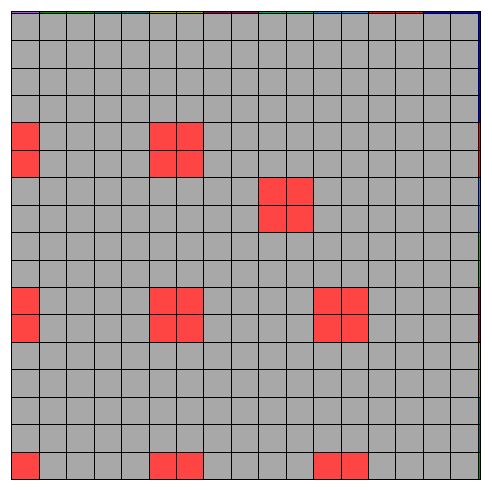
\includegraphics[width=1.5in]{problem3_radial_mat.png}
        \end{center}
      \end{figure}

      \begin{figure}[htbp!]
        \begin{center}
          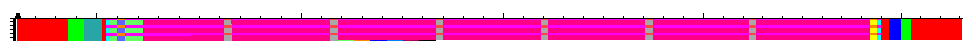
\includegraphics[width=2in]{problem3_axial_mat.png}
        \end{center}
      \end{figure}

      \begin{figure}[htpb!]
        \begin{center}
          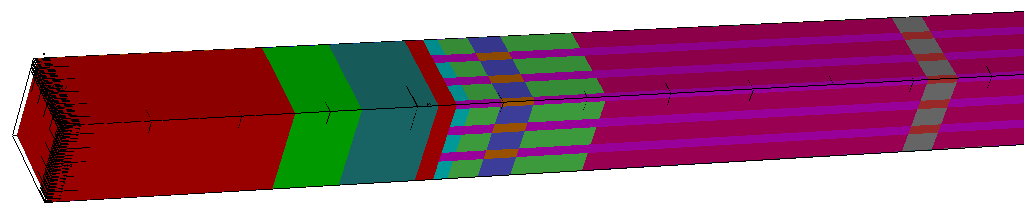
\includegraphics[width=2in]{problem3_end.png}
        \end{center}
      \end{figure}

    \end{column}

    \begin{column}{0.5\textwidth}
      {\small
        \begin{itemize}
        \item CASL Problem 3: $17 \times 17$ quarter symmetry HZP LWR
          fuel assembly
        \item Multigroup $SP_N$ discretization
        \item MCLS leveraged by the Exnihilo code base (ORNL)
        \item Emphasize algorithm development for iterative
          performance
        \end{itemize}
      }
      {\tiny
        \begin{table}[htpb!]
          \begin{center}
            \begin{tabular}{ll}\hline\hline
              \multicolumn{1}{l}{\textbf{Parameter}} & 
              \multicolumn{1}{l}{\textbf{Value}} \\
              Power Level & 0 MW \\
              Inlet Temperature & 326.85C \\
              Fuel Temperature & 600C \\
              Boron Concentration & 1300 ppm \\
              Moderator Density & 0.743 g/cc \\
              Helium Density & \sn{1.79}{-4} g/cc \\
              Zirconium Density & 6.56 g/cc \\
              Stainless Steel Density & 8.0 g/cc \\
              Inconel Density & 8.19 g/cc \\
              UO2 Density & 10.257 g/cc \\
              Fuel Pin Radius (w/o clad) & 0.4096 cm \\
              %%
              \hline\hline
            \end{tabular}
          \end{center}
        \end{table}
      }
    \end{column}

  \end{columns}

\end{frame}

%%---------------------------------------------------------------------------%%
\begin{frame}{$SP_N$ Equations}

  \begin{multline}
    \hat{\Omega} \cdot \vec{\nabla} \psi(\vec{r},\hat{\Omega},E) +
    \sigma(\vec{r},E) \psi(\vec{r},\hat{\Omega},E) = \\ \iint
    \sigma_s(\vec{r},E' \rightarrow E,\hat{\Omega}' \cdot \hat{\Omega})
    \psi(\vec{r},\hat{\Omega}',E') d\Omega' dE' +
    q(\vec{r},\hat{\Omega},E)\:,
    \label{eq:general_transport}
  \end{multline}

  \smallskip

  \begin{multline}
    -\nabla \cdot \Bigg[\frac{n}{2n+1}\frac{1}{\Sigma_{n-1}} \nabla
      \Big(\frac{n-1}{2n-1} \phi_{n-2} + \frac{n}{2n-1}\phi_n \Big) \\+
      \frac{n+1}{2n+1}\frac{1}{\Sigma_{n+1}} \nabla
      \Big(\frac{n+1}{2n+3}\phi_n + \frac{n+2}{2n+3}\phi_{n+2}\Big)
      \Bigg] \\+ \Sigma_n \phi_n = q \delta_{n0}\ \ \ \ \ \ \ \ \ n =
    0,2,4,\cdots,N\:,
    \label{eq:spn_equations}
  \end{multline}

  \smallskip

  \begin{equation}
    -\nabla \cdot \mathbb{D}_n \nabla \mathbb{U}_n + \sum_{m=1}^4
    \mathbb{A}_{nm} \mathbb{U}_m = \frac{1}{k} \sum_{m=1}^4
    \mathbb{F}_{nm} \mathbb{U}_m\ \ \ \ \ \ \ n = 1,2,3,4\:.
    \label{eq:spn_fission_matrix}
  \end{equation}

\end{frame}

%%---------------------------------------------------------------------------%%
\begin{frame}[fragile]{k-eigenvalue Solutions with MCSA}

  \begin{algorithm}[H]
    \caption{Power Iteration MCSA Scheme}
    \label{alg:power_iteration}
    \begin{algorithmic}
      \STATE $k_0 =$ initial guess
      \STATE $\mathbf{\Phi}_0 =$ initial guess
      \STATE $n = 0$
      \WHILE{$|\frac{k^n - k^{n-1}}{k^n}| > \epsilon$}
      \STATE $\mathbf{M} \mathbf{\Phi}^{n+1} = \frac{1}{k^n} \mathbf{F} \mathbf{\Phi}^n$
      \COMMENT{Solve for the new flux state with MCSA}
      \STATE $k^{n+1} = k^n \frac{\int \mathbf{F} \mathbf{\Phi}^{n+1} d\mathbf{r}}{\int
        \mathbf{F} \mathbf{\Phi}^n d\mathbf{r}}$
      \STATE $n = n+1$
      \ENDWHILE
    \end{algorithmic}
  \end{algorithm}

  \begin{itemize}
  \item Inject MCSA as the solver at each eigenvalue iteration
    \medskip
  \item Transport operator is static - one time cost for MCSA setup
    \medskip
  \item Current Exnihilo implementation gives the full operator
  \end{itemize}

\end{frame}

%%---------------------------------------------------------------------------%%
\begin{frame}{Block Jacobi Preconditioned Calculations}

{\tiny  \begin{table}[h!]
    \begin{center}
      \begin{tabular}{cccccc}\hline\hline
        \multicolumn{1}{c}{}& 
        \multicolumn{1}{c}{}& 
        \multicolumn{1}{c}{}& 
        \multicolumn{1}{c}{$SP_N$ Order}& 
        \multicolumn{1}{c}{}& 
        \multicolumn{1}{c}{} \\
        &   & \textbf{1} & \textbf{3} & \textbf{5} & \textbf{7}  \\
        & \textbf{0} & 0.0647 & 0.1275 & 0.1449 & 0.1514 \\
        & \textbf{1} & 0.0686 & 0.1338 & 0.1484 & 0.1547 \\
        $P_N$ Order & \textbf{3} & 0.0687 & 0.1399 & 0.1582 & 0.1625 \\
        & \textbf{5} & 0.0692 & 0.1399 & 0.1582 & 0.1657 \\
        & \textbf{7} & 0.0678 & 0.1393 & 0.1624 & 0.166 \\
        %%
        \hline\hline
      \end{tabular}
    \end{center}
    \caption{Spectral radius results for the block Jacobi
      preconditioned iteration matrix with 10 energy groups and full
      downscatter for sample problem.}
    \label{tab:group10dsbj}
  \end{table}
}

  \begin{columns}

    \begin{column}{0.5\textwidth}

      \begin{figure}[t!]
        \begin{center}
          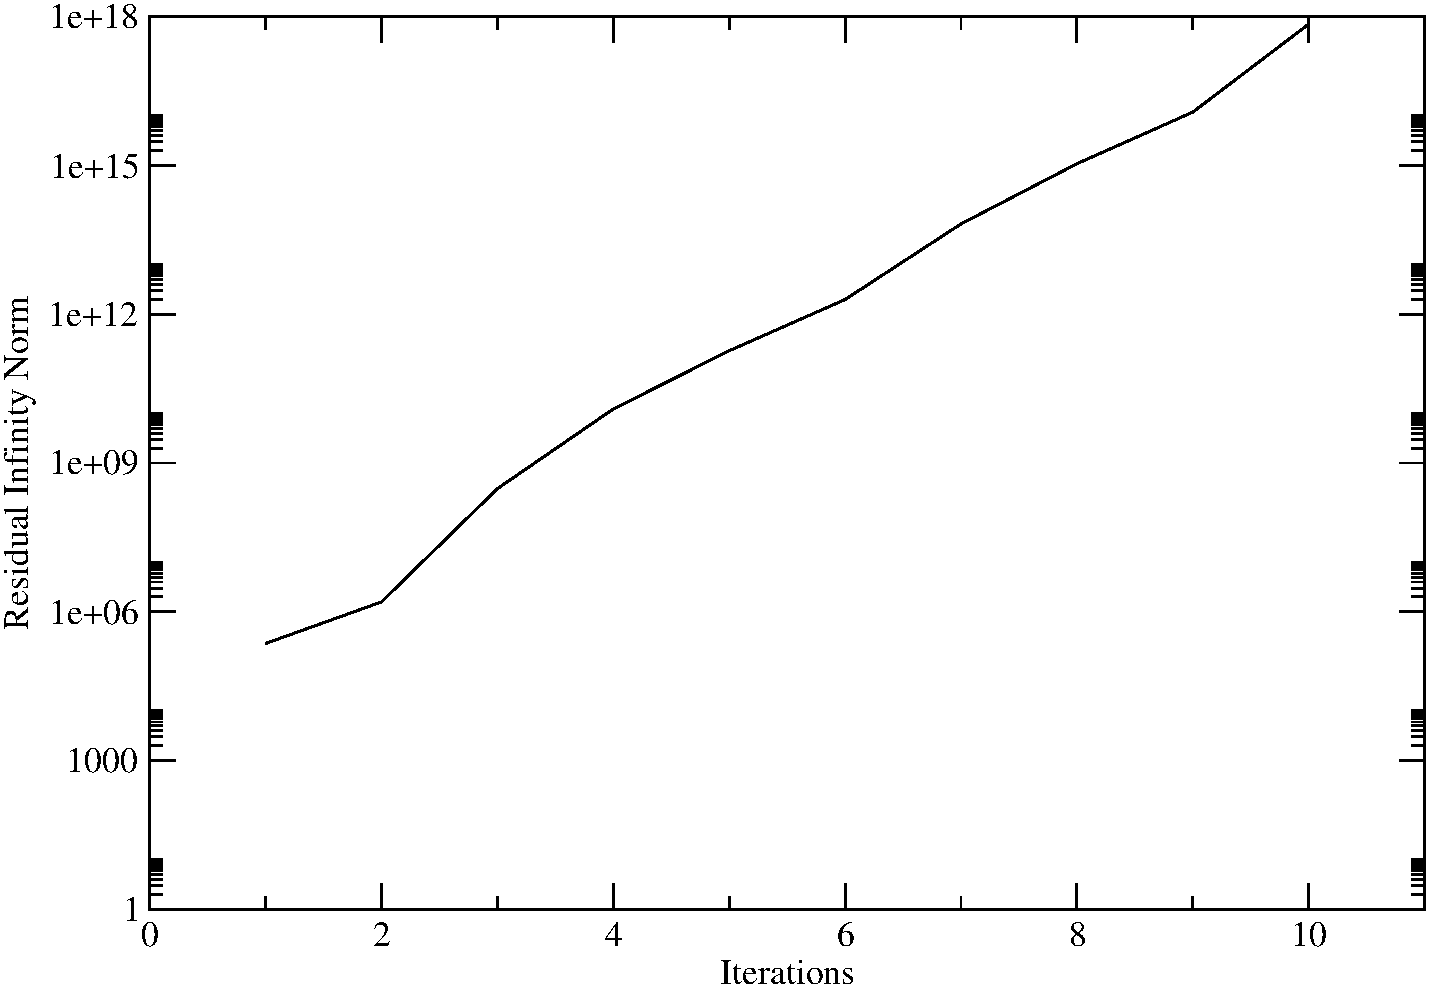
\includegraphics[width=2.0in]{block_jacobi_res.pdf}
        \end{center}
      \end{figure}

    \end{column}

    \begin{column}{0.5\textwidth}
      \begin{itemize}
      \item Rapidly divergent results
        \medskip
      \item Light water moderator creates a lot of scattering and
        $\mathbf{\rho}(\mathbf{H}) \approx 1$
        \medskip
      \item Convergence not achieved with 50 histories per DOF and 90
        minutes compute time
      \end{itemize}
    \end{column}

  \end{columns}

\end{frame}

%%---------------------------------------------------------------------------%%
\begin{frame}{MCSA Breakdown}

  \begin{columns}

    \begin{column}{0.5\textwidth}

      \begin{figure}[h!]
        \begin{center}
          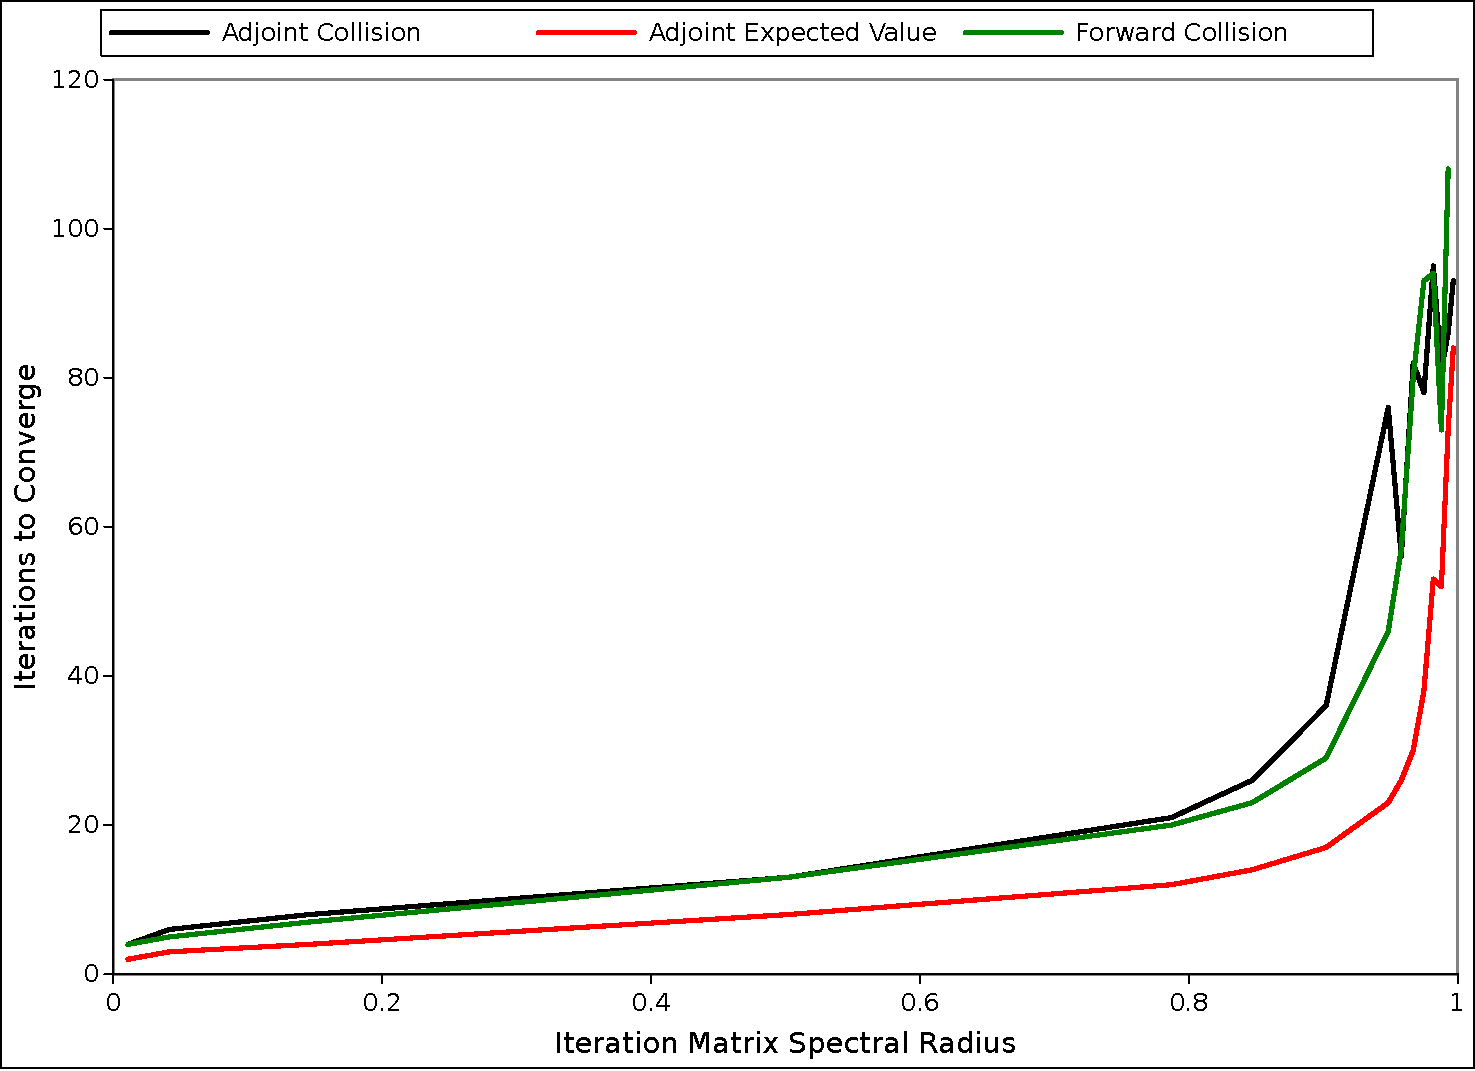
\includegraphics[width=1.9in]{breakdown_iterations.pdf}
        \end{center}
      \end{figure}

      \begin{figure}[h!]
        \begin{center}
          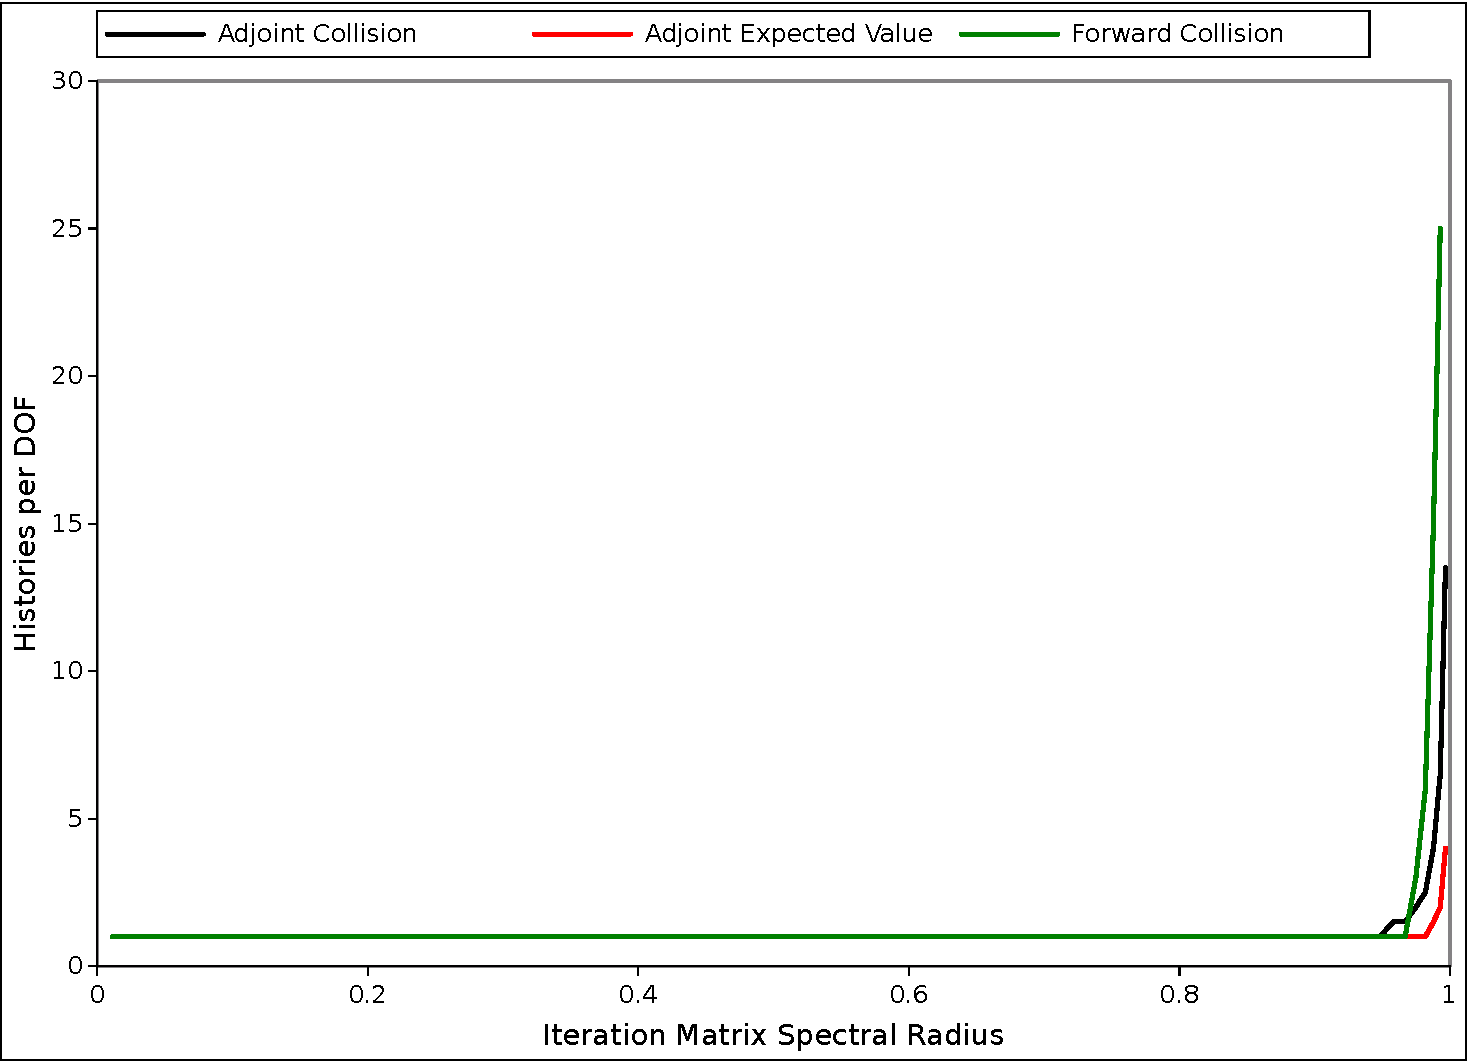
\includegraphics[width=1.9in]{breakdown_histories.pdf}
        \end{center}
      \end{figure}

    \end{column}

    \begin{column}{0.5\textwidth}

    \begin{itemize}
    \item As $\mathbf{\rho}(\mathbf{H}) \rightarrow 1$ terrible things
      happen...
      \medskip
    \item A more robust set of preconditioners is required for the
      $SP_N$ equations
    \end{itemize}

      \begin{figure}[h!]
        \begin{center}
          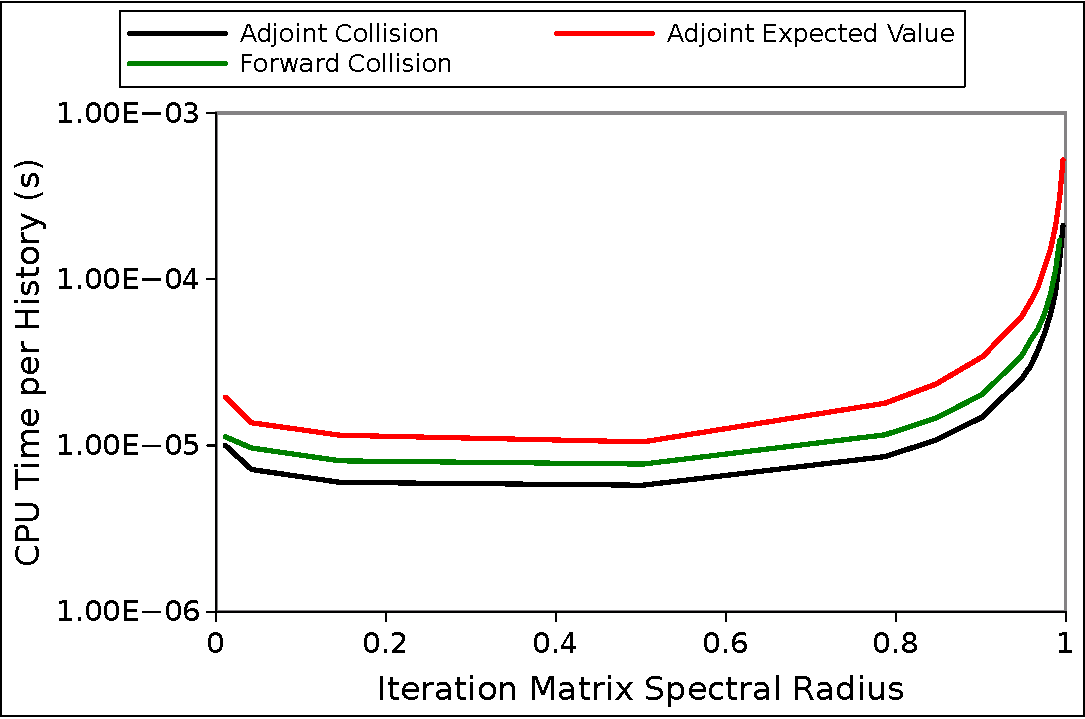
\includegraphics[width=1.9in]{breakdown_time.pdf}
        \end{center}
      \end{figure}

    \end{column}

  \end{columns}

\end{frame}

%%---------------------------------------------------------------------------%%
\begin{frame}{Explicit Preconditioning}

  \[
  \ve{M}_L^{-1}\ve{A}\ve{M}_R^{-1}\ve{M}_R\ve{x} = \ve{M}_L^{-1}\ve{b}
  \ \ \ \rightarrow \ \ \ 
  \ve{M}_L^{-1}\ve{A}\ve{M}_R^{-1}\ve{u} = \ve{M}_L^{-1}\ve{b}
  \]

  \[
  \ve{x} = \ve{M}_R^{-1}\ve{u}
  \]

  \begin{beamerboxesrounded}[upper=boxheadcolor,lower=boxbodycolor,shadow=true]
    {Left/Right Preconditioned MCSA Iteration}

    \[
    \ve{r}^{k} = \ve{M}_L^{-1}(\ve{b}-\ve{A}\ve{M}_R^{-1}\ve{u}^{k})
    \]
    \[
    \ve{u}^{k+1/2} = \ve{u}^k + \ve{r}^k
    \]
    \[
    \ve{r}^{k+1/2} = \ve{M}_L^{-1}(\ve{b}-\ve{A}\ve{M}_R^{-1}\ve{u}^{k+1/2})
    \]
    \[
    \ve{M}_L^{-1}\ve{A}\ve{M}_R^{-1}\delta\ve{u}^{k+1/2} = \ve{r}^{k+1/2}
    \]
    \[
    \ve{u}^{k+1} = \ve{u}^{k+1/2} + \delta \ve{u}^{k+1/2}
    \]

  \end{beamerboxesrounded}

\end{frame}

%%---------------------------------------------------------------------------%%
\begin{frame}{ILUT Preconditioning}

  \begin{columns}

    \begin{column}{0.5\textwidth}

      \begin{figure}[t!]
        \begin{center}
          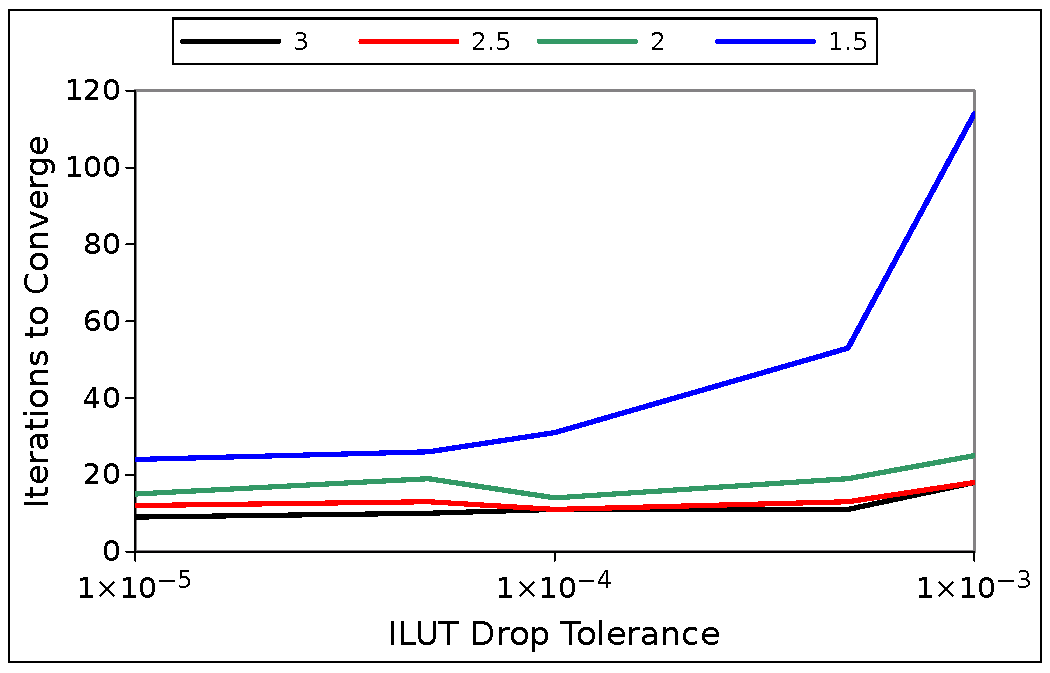
\includegraphics[width=2.0in]{ilut_iterations.pdf}
        \end{center}
      \end{figure}

      \begin{figure}[t!]
        \begin{center}
          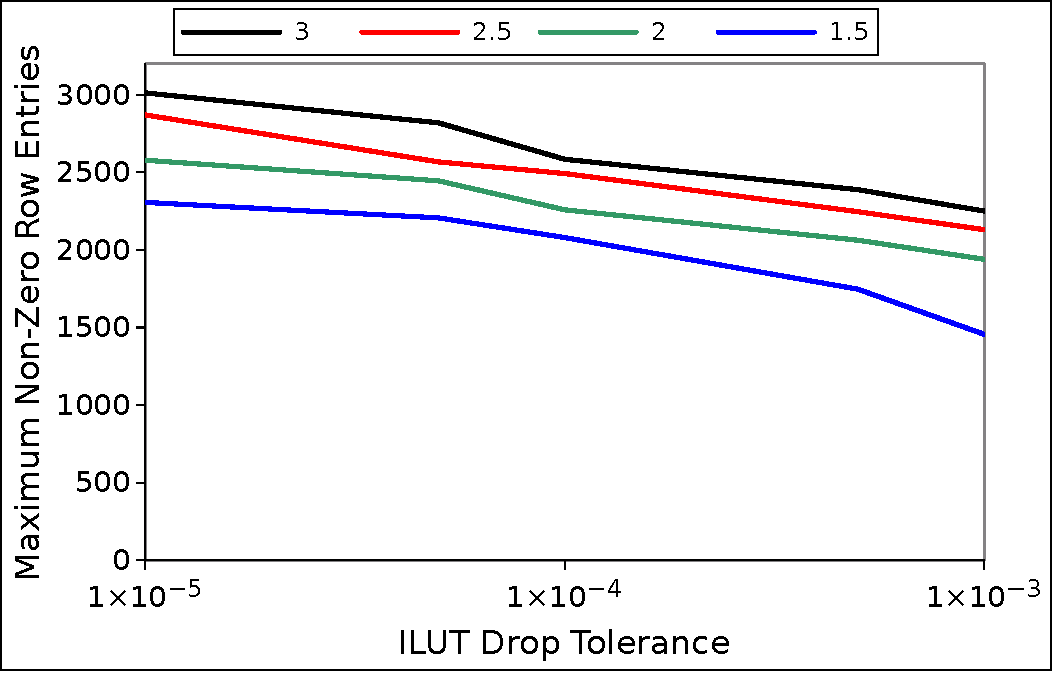
\includegraphics[width=2.0in]{ilut_size.pdf}
        \end{center}
      \end{figure}

    \end{column}

    \begin{column}{0.5\textwidth}

      \begin{itemize}
      \item {\small Factor transport operator into upper and lower
        triangular parts}
        \begin{itemize}
        \item {\small $\mathbf{R} = \mathbf{L} \mathbf{U} -
          \mathbf{M}$}
        \end{itemize}
      \item {\small Control factorization content with level-of-fill
        and drop tolerance}
      \item {\small Use the reduced domain approximation to recover
        sparsity}
      \end{itemize}

      \begin{figure}[t!]
        \begin{center}
          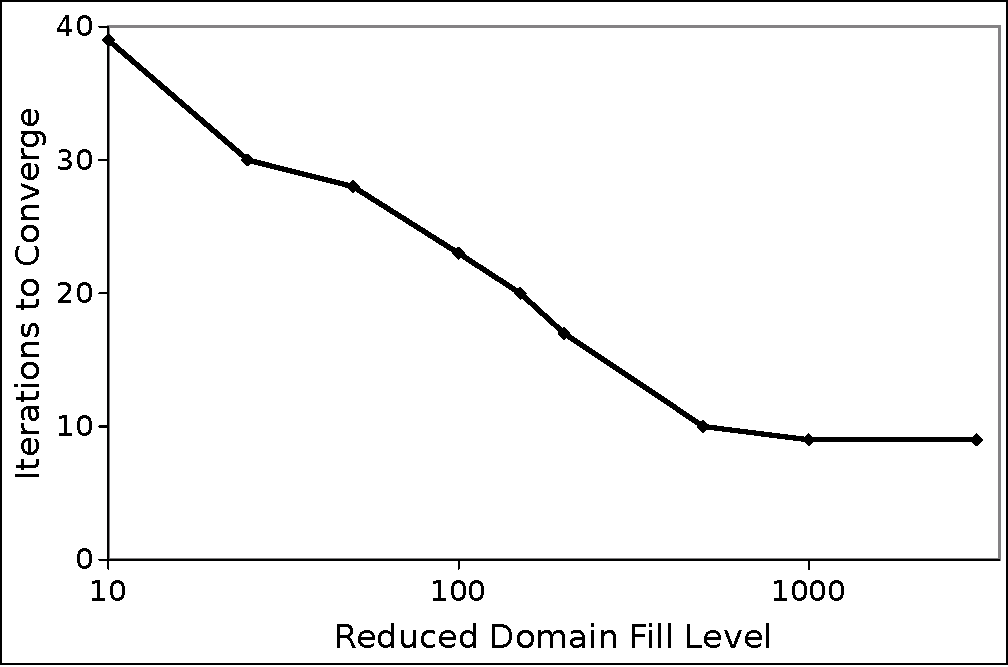
\includegraphics[width=2.0in]{rda_ilut_iterations.pdf}
        \end{center}
      \end{figure}

    \end{column}


  \end{columns}

\end{frame}

%%---------------------------------------------------------------------------%%
\begin{frame}{Fuel Assembly Results}

  \begin{columns}

    \begin{column}{0.5\textwidth}

      {\tiny
      \begin{table}[h!]
        \begin{center}
          \begin{tabular}{lccc}\hline\hline
            \multicolumn{1}{l}{Solver}&
            \multicolumn{1}{c}{1 Group}&
            \multicolumn{1}{c}{2 Groups}&
            \multicolumn{1}{c}{4 Groups}\\
            \hline
            BiCGStab-ILUT & 11.6 & 11.6 & 12.4 \\ 
            GMRES-ILUT & 18.1 & 17.9 & 18.9 \\
            MCSA-ILUT-R-C & 14.6 & 15.4 & 17.6 \\
            MCSA-ILUT-MR-C & 16.0 & 17.1 & 23.7 \\
            MCSA-ILUT-R-EV & 18.3 & 19.4 & 16.8 \\
            MCSA-ILUT-MR-EV & 19.6 & 22.4 & 17.5 \\
            Richardson-ILUT & 60.9 & 60.4 & 63.4 \\
            %%
            \hline\hline
          \end{tabular}
        \end{center}
        \caption{Average number of linear solver iterations per
          eigenvalue iteration.}
      \end{table}
      }

      \begin{figure}[htpb!]
        \begin{center}
          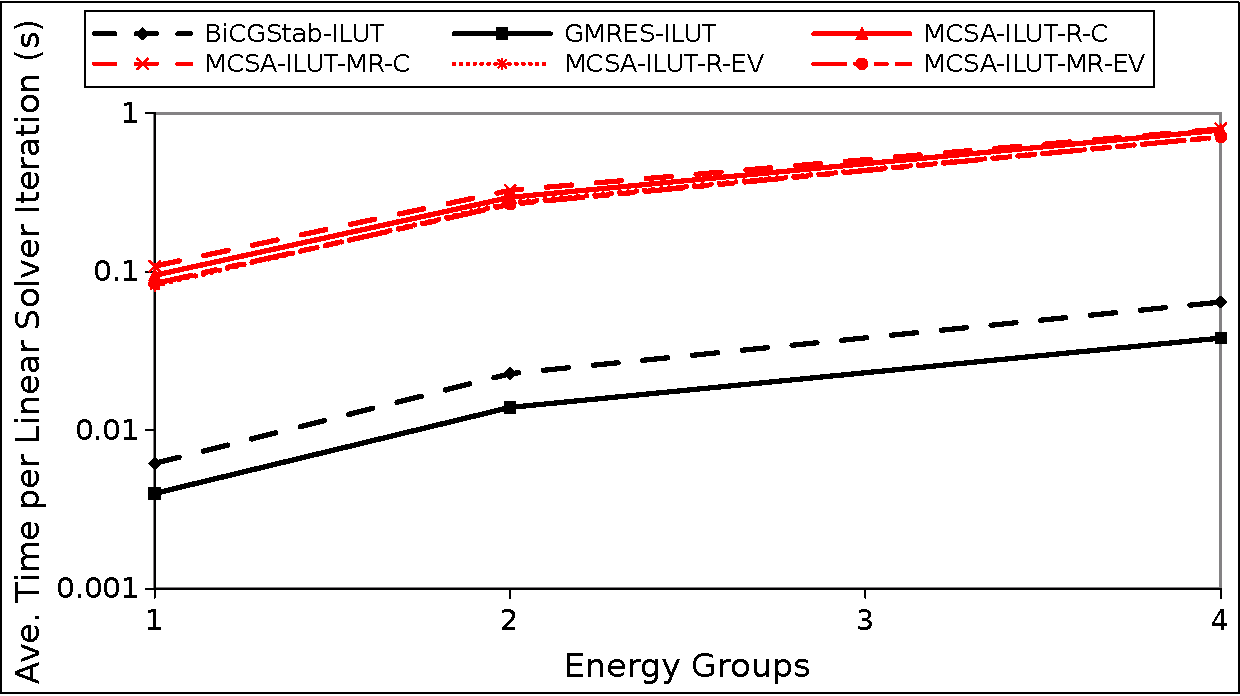
\includegraphics[width=2.25in]{solver_time.pdf}
        \end{center}
      \end{figure}

    \end{column}

    \begin{column}{0.5\textwidth}
      
      \begin{itemize}
        {\small
        \item Comparison to Trilinos Aztec Krylov solvers with ILUT
          \medskip
        \item MCLS verified for the k-eigenvalue and neutron flux in
          all groups
          \medskip
        \item MCSA converged in fewer iterations than GMRES, more
          iterations than BiCGStab
          \medskip
        \item Explicit preconditioning strategy destroys sparsity and
          elevates CPU times (Ifpack ILUT)
          \medskip
        \item Spectral radius and memory limitations combine to
          prevent solutions at finer discretizations
        }
      \end{itemize}

    \end{column}

  \end{columns}

\end{frame}

%%---------------------------------------------------------------------------%%
\begin{frame}{Outline}

  \begin{itemize}
  \item Introduction
    \bigskip
  \item Monte Carlo Synthetic Acceleration Methods
    \bigskip
  \item Application to Neutron Transport
    \bigskip
  \item \textbf{Application to Fluid Flow}
    \bigskip
  \item Parallelization of MCSA
    \bigskip
  \item Summary
  \end{itemize}

\end{frame}

%%---------------------------------------------------------------------------%%
\begin{frame}{Navier-Stokes Benchmark Problems}

  \begin{itemize}
  \item Sequence of Navier-Stokes benchmarks
    \begin{itemize}
    \item Thermal convection cavity problem (De Vahl Davis, 1983)
    \item Lid driven cavity problem (Ghia et al., 1982)
    \item Backward-Facing step problem (Gartling, 1990)
    \end{itemize}
    \medskip
  \item Tuning benchmark parameters varies the strength of
    nonlinearities
  \end{itemize}

  \begin{columns}
    \begin{column}{0.4\textwidth}
      {\small
      \[
      \rho \ve{u} \cdot \nabla \ve{u} - \nabla \cdot \ve{T} - \rho
      \ve{g} = \ve{0}
      \]
      \[
      \nabla \cdot \ve{u} = 0
      \]
      \[
      \rho C_p \ve{u} \cdot \nabla T + \nabla \cdot \ve{q} = 0
      \]
      \[
      \ve{T} = -P \ve{I} + \mu[\nabla \ve{u} + \nabla \ve{u}^T]
      \]
      \[
      \ve{q} = - k \nabla T
      \]
      }
    \end{column}

    \begin{column}{0.6\textwidth}

      \begin{figure}[htpb!]
        \begin{center}
          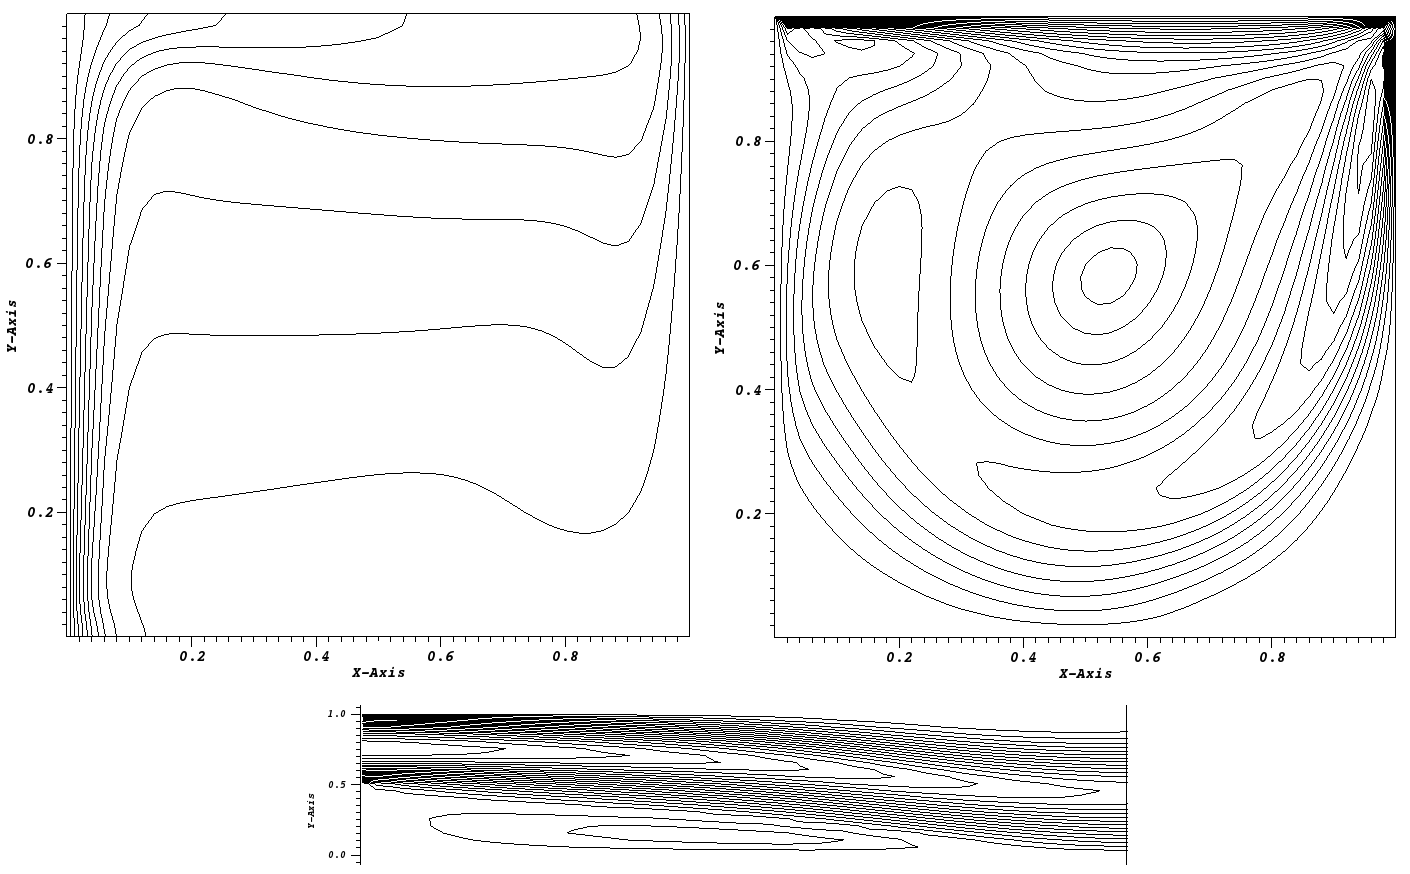
\includegraphics[width=2.9in]{benchmark_solutions.png}
        \end{center}
      \end{figure}

    \end{column}
  \end{columns}

\end{frame}

%%----------s-----------------------------------------------------------------%%
\begin{frame}{MCSA for the Navier-Stokes Equations}

  \begin{itemize}
  \item Need a nonlinear solution scheme for the Navier-Stokes equations
    \bigskip
  \item Significant research on Newton methods since the 1980's
    \bigskip
  \item Newton methods often leverage Krylov solvers
    \begin{itemize}
    \item Simple implementation
    \item No operator required
    \end{itemize}
    \bigskip
  \item Monte Carlo methods need the full operator
    \bigskip
  \item Automatic construction of the linear model is available
    \begin{itemize}
    \item Operator overloading for nonlinear residual differentiation
    \item Ideal for Monte Carlo
    \item Similar framework properties to matrix-free methods
    \end{itemize}
  \end{itemize}

\end{frame}

%%---------------------------------------------------------------------------%%
\begin{frame}{Newton's Method}

  \begin{itemize}
  \item Seek solutions of the general nonlinear problem
  \end{itemize}

  \[
  \ve{F}(\ve{u}) = \ve{0}
  \]
  \[
  \ve{u} \in \mathbb{R}^n,\ \ve{F}:\mathbb{R}^N \rightarrow
  \mathbb{R}^N
  \]

  \begin{itemize}
  \item Interpret the exact solution $\ve{u}$ to be the roots of
    $\ve{F}(\ve{u})$
  \end{itemize}

  \[
  \ve{F}(\ve{u}^{k+1}) = \ve{F}(\ve{u}^{k}) +
  \ve{F}'(\ve{u}^{k})(\ve{u}^{k+1}-\ve{u}^{k}) +
  \frac{\ve{F}''(\ve{u}^{k})}{2}(\ve{u}^{k+1}-\ve{u}^{k})^2 + \cdots
  \]

  \begin{itemize}
  \item Form Newton's method
  \end{itemize}
  \[
  \ve{J}(\ve{u}) \delta \ve{u}^k = -\ve{F}(\ve{u}^{k})
  \]
  \[
  \ve{u}^{k+1} = \ve{u}^k + \delta \ve{u}^k
  \]

\end{frame}

%%---------------------------------------------------------------------------%%
\begin{frame}[fragile]{The FANM Method}

  Forward-Automated Newton-MCSA

  \begin{algorithm}[H]
    \begin{algorithmic}[1]
      \STATE $k := 0$ 
      \WHILE{$||\ve{F}(\ve{u}^{k})|| > \epsilon
        ||\ve{F}(\ve{u}^{0})||$} 
      \STATE $\ve{J}(\ve{u}^{k}) \leftarrow AD(\ve{F}(\ve{u}^k))$ 
      \COMMENT{Automatic differentiation} 
      \STATE $\ve{J}(\ve{u}^k) \delta \ve{u}^k = -\ve{F}(\ve{u}^{k})$
      \COMMENT{Solve for the Newton correction with MCSA} 
      \STATE $\ve{u}^{k+1} \leftarrow \ve{u}^k + \delta \ve{u}^k$ 
      \STATE $k \leftarrow k+1$ 
      \ENDWHILE
    \end{algorithmic}
    \caption{FANM}
  \end{algorithm}

  \begin{itemize}
  \item Robustness of Newton's method (inexact)
  \item Accuracy and convenience of FAD
  \item Potential parallelism, and resiliency benefits of MCSA
  \item Requires only nonlinear function evaluations
  \item Can utilize globalization and forcing term selection methods
  \end{itemize}


\end{frame}

%%---------------------------------------------------------------------------%%
\begin{frame}{FANM Numerical Experiments}

  \begin{columns}
    \begin{column}{0.5\textwidth}
      \begin{figure}[htpb!]
        \begin{center}
          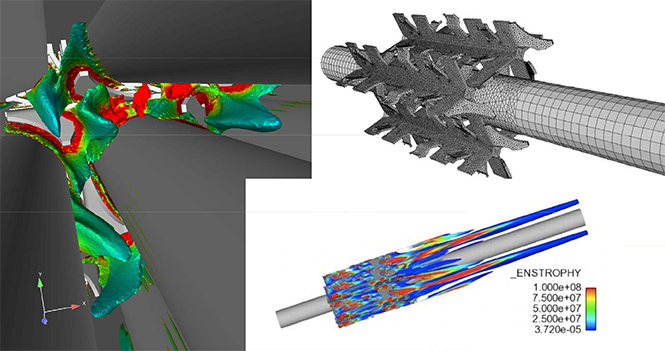
\includegraphics[width=2.0in]{drekar1.png}
        \end{center}
      \end{figure}
    \end{column}

    \begin{column}{0.5\textwidth}
      \begin{figure}[htpb!]
        \begin{center}
          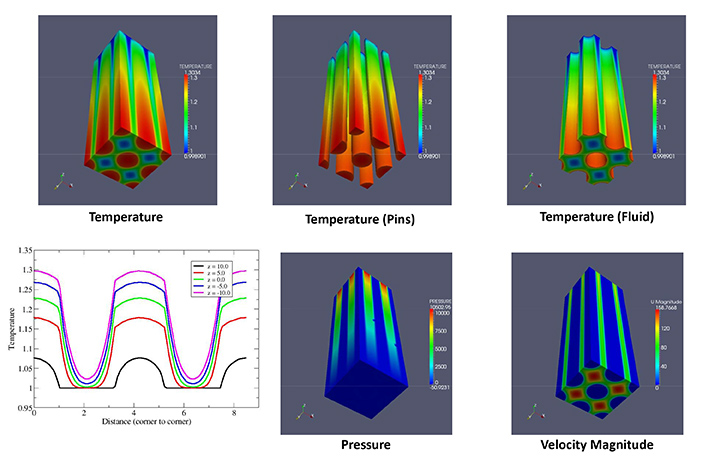
\includegraphics[width=2.0in]{drekar2.png}
        \end{center}
      \end{figure}
    \end{column}
  \end{columns}

  \medskip

  \begin{itemize}
    {\small
    \item Drekar is a production CFD code using Newton methods with
      FAD
      \medskip
    \item MCLS incorporated into Drekar nonlinear scheme to implement
      FANM
      \medskip
    \item Newton-Krylov method with Aztec GMRES used for benchmark
      comparisons
    \item All methods and problems preconditioned with explicit scheme
      using algebraic multigrid (ML) and leveraged some kind of
      globalization (e.g. backtracking) with RDA
    }
  \end{itemize}

  {\small \sl Images source: www.casl.gov}

\end{frame}

%%---------------------------------------------------------------------------%%
\begin{frame}{Thermal Convection Cavity Results}

  \begin{columns}
    \begin{column}{0.6\textwidth}

      \small{
        \begin{table}[h!]
          \begin{center}
            \begin{tabular}{lccc}\hline\hline
              \multicolumn{1}{l}{Benchmark}& 
              \multicolumn{1}{c}{NK}&
              \multicolumn{1}{c}{FANM}&
              \multicolumn{1}{c}{NR}\\
              \hline
              Ra=\sn{1}{3} & 5 & 5 & 5\\
              Ra=\sn{1}{4} & 7 & 7 & 7\\
              Ra=\sn{1}{5} & 9 & 10 & 9\\
              Ra=\sn{1}{6} & 11 & 11 & 11\\
              %%
              \hline\hline
            \end{tabular}`
          \end{center}
          \caption{Nonlinear iterations.}
        \end{table}

        \begin{table}[h!]
          \begin{center}
            \begin{tabular}{lccc}\hline\hline
              \multicolumn{1}{l}{Benchmark}& 
              \multicolumn{1}{c}{GMRES}&
              \multicolumn{1}{c}{MCSA}&
              \multicolumn{1}{c}{Richardson}\\
              \hline
              Ra=\sn{1}{3} & 32 & 18 & 38\\
              Ra=\sn{1}{4} & 23 & 17 & 34\\
              Ra=\sn{1}{5} & 25 & 20 & 34\\
              Ra=\sn{1}{6} & 39 & 25 & 48\\
              %%
              \hline\hline
            \end{tabular}
          \end{center}
          \caption{Total linear solver iterations.}
        \end{table}
      }

    \end{column}

    \begin{column}{0.4\textwidth}

      \small{
        \begin{itemize}
        \item Weaker preconditioning at Ra=\sn{1}{5} case
          \medskip
        \item Constant forcing term for Ra=\sn{1}{6} case
        \end{itemize}
      }

      \bigskip

      \tiny{
        \begin{table}[h!]
          \begin{center}
            \begin{tabular}{lc}\hline\hline
              \multicolumn{1}{l}{Benchmark}& 
              \multicolumn{1}{c}{NK Speedup}\\
              \hline
              Ra=\sn{1}{3} & 338 \\
              Ra=\sn{1}{4} & 336 \\
              Ra=\sn{1}{5} & 346 \\
              Ra=\sn{1}{6} & 465 \\
              \hline\hline
            \end{tabular}
          \end{center}
          \caption{Newton-Krylov speedup over FANM.}
        \end{table}
      }

    \end{column}
  \end{columns}

\end{frame}

%%---------------------------------------------------------------------------%%
\begin{frame}{Lid Driven Cavity Results}

  \begin{columns}
    \begin{column}{0.6\textwidth}

      \small{
        \begin{table}[h!]
          \begin{center}
            \begin{tabular}{lccc}\hline\hline
              \multicolumn{1}{l}{Benchmark}& 
              \multicolumn{1}{c}{NK}&
              \multicolumn{1}{c}{FANM}&
              \multicolumn{1}{c}{NR}\\
              \hline
              Re=100 & 6 & 6 & 7\\
              Re=300 & 9 & 9 & 9\\
              Re=500 & 11 & 11 & 11\\
              Re=700 & 14 & 10 & 12\\
              %%
              \hline\hline
            \end{tabular}`
          \end{center}
          \caption{Nonlinear iterations.}
        \end{table}

        \begin{table}[h!]
          \begin{center}
            \begin{tabular}{lccc}\hline\hline
              \multicolumn{1}{l}{Benchmark}& 
              \multicolumn{1}{c}{GMRES}&
              \multicolumn{1}{c}{MCSA}&
              \multicolumn{1}{c}{Richardson}\\
              \hline
              Re=100 & 27 & 42 & 151\\
              Re=300 & 35 & 52 & 133\\
              Re=500 & 41 & 56 & 154\\
              Re=700 & 21 & 14 & 32\\
              %%
              \hline\hline
            \end{tabular}
          \end{center}
          \caption{Total linear solver iterations.}
        \end{table}
      }

    \end{column}

    \begin{column}{0.4\textwidth}

      \small{
        \begin{itemize}
        \item $\eta_k = \gamma \Big(
          \frac{||\ve{F}(\ve{u}_k)||}{||\ve{F}(\ve{u}_{k-1})||}
          \Big)^{\alpha}$
        \item Newton-Krylov always had larger forcing terms
        \item At Re=700, MCSA histories doubled and RDA fill increased
          from 200 to 300
        \end{itemize}
      }

      \smallskip

      \tiny{
        \begin{table}[h!]
          \begin{center}
            \begin{tabular}{lc}\hline\hline
              \multicolumn{1}{l}{Benchmark}& 
              \multicolumn{1}{c}{NK Speedup}\\
              \hline
              Re=100 & 299 \\
              Re=300 & 322 \\
              Re=500 & 288 \\
              Re=700 & 488 \\
              %%
              \hline\hline
            \end{tabular}
          \end{center}
          \caption{Newton-Krylov speedup over FANM.}
        \end{table}
      }

    \end{column}
  \end{columns}

\end{frame}

%%---------------------------------------------------------------------------%%
\begin{frame}{Backward Facing Step Results}

  \begin{columns}
    \begin{column}{0.6\textwidth}

      \small{
        \begin{table}[h!]
          \begin{center}
            \begin{tabular}{lccc}\hline\hline
              \multicolumn{1}{l}{Benchmark}& 
              \multicolumn{1}{c}{NK}&
              \multicolumn{1}{c}{FANM}&
              \multicolumn{1}{c}{NR}\\
              \hline
              Re=200 & 10 & 9 & 10\\
              Re=300 & 15 & 14 & 15\\
              Re=400 & 10 & 10 & 10\\
              Re=500 & 19 & 20 & 21\\
              %%
              \hline\hline
            \end{tabular}`
          \end{center}
          \caption{Nonlinear iterations.}
        \end{table}

        \begin{table}[h!]
          \begin{center}
            \begin{tabular}{lccc}\hline\hline
              \multicolumn{1}{l}{Benchmark}& 
              \multicolumn{1}{c}{GMRES}&
              \multicolumn{1}{c}{MCSA}&
              \multicolumn{1}{c}{Richardson}\\
              \hline
              Re=200 & 24 & 13 & 21\\
              Re=300 & 23 & 17 & 21\\
              Re=400 & 18 & 12 & 14\\
              Re=500 & 30 & 52 & 98\\
              %%
              \hline\hline
            \end{tabular}
          \end{center}
          \caption{Total linear solver iterations.}
        \end{table}
      }

    \end{column}

    \begin{column}{0.4\textwidth}

      \begin{itemize}
      \item Significantly more ill-conditioned than cavity problems
      \item Forcing terms are not the culprit
      \item Multigrid is doing significantly more work
      \end{itemize}

      \bigskip

      \tiny{
        \begin{table}[h!]
          \begin{center}
            \begin{tabular}{lc}\hline\hline
              \multicolumn{1}{l}{Benchmark}& 
              \multicolumn{1}{c}{NK Speedup}\\
              \hline
              Re=200 & 400 \\
              Re=300 & 593 \\
              Re=400 & 825 \\
              Re=500 & 1057 \\
              %%
              \hline\hline
            \end{tabular}
          \end{center}
          \caption{Newton-Krylov speedup over FANM.}
        \end{table}
      }

    \end{column}
  \end{columns}

\end{frame}

%%---------------------------------------------------------------------------%%
\begin{frame}{FANM Iterative Performance Summary}

  {\tiny

    \begin{columns}
      \begin{column}{0.5\textwidth}

        \begin{table}[h!]
          \begin{center}
            \begin{tabular}{lcc}\hline\hline
              \multicolumn{1}{l}{Benchmark}& 
              \multicolumn{1}{c}{Newton-Krylov}&
              \multicolumn{1}{c}{FANM}\\
              \hline
              Convection, Ra=\sn{1}{3} & $\times$ & $\times$ \\
              Convection, Ra=\sn{1}{4} & $\times$ & $\times$ \\
              Convection, Ra=\sn{1}{5} & $\times$ & \\
              Convection, Ra=\sn{1}{6} & $\times$ & $\times$ \\
              Lid Driven, Re=100 & $\times$ & $\times$ \\
              Lid Driven, Re=300 & $\times$ & $\times$ \\
              Lid Driven, Re=500 & $\times$ & $\times$ \\
              Lid Driven, Re=700 & & $\times$ \\
              Backward Step, Re=200 & & $\times$ \\
              Backward Step, Re=300 & & $\times$ \\
              Backward Step, Re=400 & $\times$ & $\times$ \\
              Backward Step, Re=500 & $\times$ & \\
              %%
              \hline\hline
            \end{tabular}
          \end{center}
          \caption{Navier-Stokes benchmark comparison for nonlinear
            iterations.}
        \end{table}

      \end{column}

      \begin{column}{0.5\textwidth}

        \begin{table}[h!]
          \begin{center}
            \begin{tabular}{lcc}\hline\hline
              \multicolumn{1}{l}{Benchmark}& 
              \multicolumn{1}{c}{Newton-Krylov}&
              \multicolumn{1}{c}{FANM}\\
              \hline
              Convection, Ra=\sn{1}{3} & & $\times$ \\
              Convection, Ra=\sn{1}{4} & & $\times$ \\
              Convection, Ra=\sn{1}{5} & & $\times$ \\
              Convection, Ra=\sn{1}{6} & & $\times$ \\
              Lid Driven, Re=100 & $\times$ & \\
              Lid Driven, Re=300 & $\times$ & \\
              Lid Driven, Re=500 & $\times$ & \\
              Lid Driven, Re=700 & & $\times$ \\
              Backward Step, Re=200 & & $\times$ \\
              Backward Step, Re=300 & & $\times$ \\
              Backward Step, Re=400 & & $\times$ \\
              Backward Step, Re=500 & $\times$ & \\
              %%
              \hline\hline
            \end{tabular}
          \end{center}
          \caption{Navier-Stokes benchmark comparison for total
            linear solver iterations.}
        \end{table}

      \end{column}
    \end{columns}
  }

  {\small
    \begin{itemize}
    \item Over all benchmarks, FANM performed better in terms of nonlinear
      iterations for 1 more case than the Newton-Krylov method
      \medskip
    \item Over all benchmarks, FANM performed better in terms of linear
      solver iterations for twice as many cases as the Newton-Krylov
      method
    \end{itemize}
  }

\end{frame}

%%---------------------------------------------------------------------------%%
\begin{frame}{Outline}

  \begin{itemize}
  \item Introduction
    \bigskip
  \item Monte Carlo Synthetic Acceleration Methods
    \bigskip
  \item Application to Neutron Transport
    \bigskip
  \item Application to Fluid Flow
    \bigskip
  \item \textbf{Parallelization of MCSA}
    \bigskip
  \item Summary
  \end{itemize}

\end{frame}

%%---------------------------------------------------------------------------%%
\begin{frame}{Parallelization of Monte Carlo Methods}

  \begin{itemize}
  \item No literature observed for parallel Neumann-Ulam solvers
    beyond history-level parallelism
    \medskip \medskip
  \item Numerous references for modern parallel Monte Carlo methods in
    reactor physics
    \medskip \medskip
  \item Build a strategy for applying modern methods to the
    Neumann-Ulam method
    \medskip \medskip
  \item MCSA iteration-level parallelism comes from parallel
    matrix/vector operations
  \end{itemize}

\end{frame}

%%---------------------------------------------------------------------------%%
\begin{frame}{Domain Decomposed Monte Carlo}

  \begin{columns}
    \begin{column}{0.5\textwidth}
      \begin{itemize}
      \item Each parallel process owns a piece of the domain (linear
        system)
        \bigskip
      \item Random walks must be transported between adjacent domains
        through parallel communication
        \bigskip
      \item Domain decomposition determined by the input system
      \end{itemize}
    \end{column}

    \begin{column}{0.5\textwidth}
      \begin{figure}[htpb!]
        \begin{center}
          \scalebox{0.75}{ \input{ddnu_example.pdftex_t} }
        \end{center}
        \caption{\small Domain decomposition example illustrating
          how domain-to-domain transport creates communication costs.}
      \end{figure}
    \end{column}
  \end{columns}

\end{frame}

%%---------------------------------------------------------------------------%%
\begin{frame}{Asynchronous Monte Carlo Transport Kernel}

  \begin{columns}

    \begin{column}{0.5\textwidth}

      \begin{itemize}
      \item Developed by Brunner and Brantley in 2009
      \item Asynchronous nearest neighbor communication of histories
      \item Binary asynchronous communication tree for completing
        transport
      \end{itemize}

      \begin{figure}[htpb!]
        \begin{center}
          \scalebox{0.45}{ \input{domain_to_domain.pdftex_t} }
        \end{center}
      \end{figure}

    \end{column}

    \begin{column}{0.5\textwidth}

      \begin{itemize}
      \item Extensible to problems where histories may be created
        (i.e. variance reduction)
      \end{itemize}

      \begin{figure}[htpb!]
        \begin{center}
          \scalebox{0.45}{ \input{binary_comm_tree.pdftex_t} }
        \end{center}
      \end{figure}

    \end{column}


  \end{columns}

  \let\thefootnote\relax\footnote{\tiny{Thomas A. Brunner and Patrick
      S. Brantley, "An efficient, robust, domain-decomposition
      algorithm for particle Monte Carlo", Journal of Computational
      Physics, vol. 228, pp.3882-3890, 2009.}}
\end{frame}

%%---------------------------------------------------------------------------%%
\begin{frame}[fragile]{Multiple-Set Overlapping-Domain Decomposition}

  \begin{columns}

    \begin{column}{0.52\textwidth}

      \begin{figure}[t!]
        \begin{center}
          \scalebox{0.275}{ \input{msod_construction.pdftex_t} }
        \end{center}
        \caption{\small MSOD construction.}
      \end{figure}

    \end{column}

    \begin{column}{0.48\textwidth}

      \begin{figure}[t!]
        \begin{center}
          \scalebox{0.2}{ \input{msod_tally.pdftex_t} }
        \end{center}
        \caption{\small MSOD tally reduction.}
      \end{figure}

      \begin{itemize}
        {\small
        \item Multiple sets replicate the domain
        \item Domains overlap within a set
        \item Each set contains the full domain
        }
      \end{itemize}

    \end{column}

  \end{columns}


  \let\thefootnote\relax\footnote{\tiny{Wagner et. al., "Hybrid and
      parallel domain-decomposition methods development to enable
      Monte Carlo for reactor analysis", Joint International
      Conference on Supercomputing in Nuclear Applications and Monte
      Carlo (SNA+MC 2010), 2010.}}

\end{frame}

%%---------------------------------------------------------------------------%%
\begin{frame}{Leadership-Class Parallel Scaling Studies}

  \begin{itemize}
  \item Simple 2D neutron diffusion problem for control - spectral
    radius is maintained as global problem size grows
    \medskip
  \item Comparison to Trilinos Belos Krylov solvers with Jacobi
    preconditioning - conjugate gradient and GMRES
    \medskip
  \item Strong scaling - Global size fixed at 1.6E7 DOFs
    \medskip
  \item Weak scaling - Local size fixed at 4.0E4 DOFs
    \medskip
  \item Calculations performed on the Titan Cray XK7 machine at ORNL
    (MPI only)
    \medskip
  \item Limited MCLS arithmetic optimization artificially inflates
    efficiencies
  \end{itemize}

\end{frame}

%%---------------------------------------------------------------------------%%
\begin{frame}{Strong Scaling Results}

  \begin{columns}

    \begin{column}{0.5\textwidth}

      \begin{figure}[htpb!]
        \begin{center}
          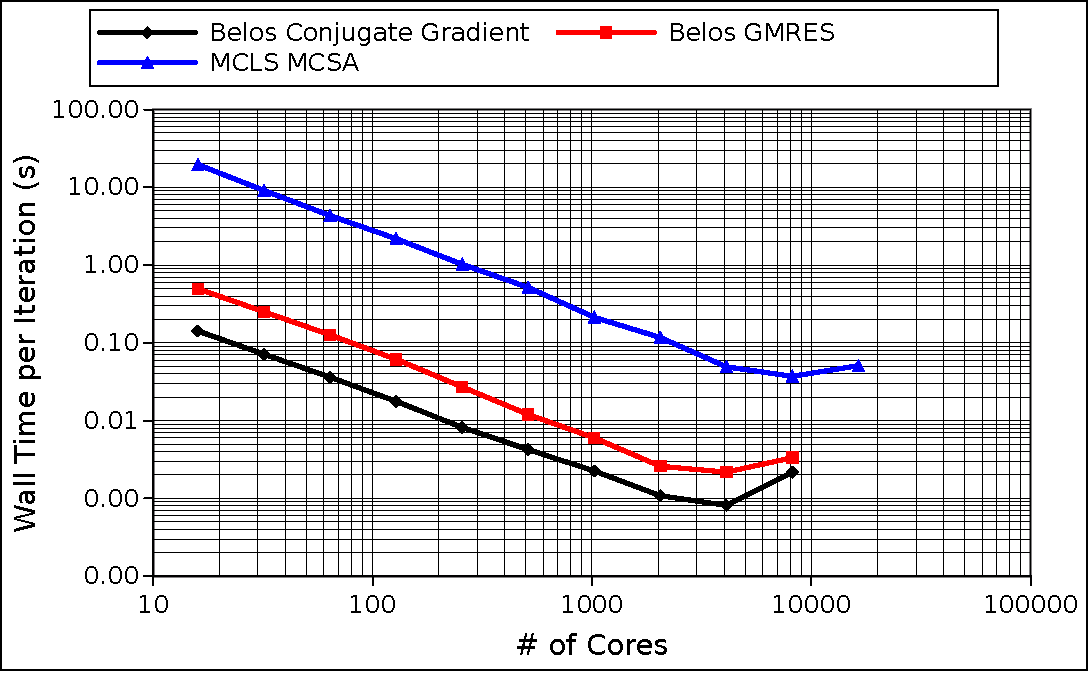
\includegraphics[width=2.4in]{titan_pure_strong_time.pdf}
        \end{center}
        \caption{Wall time.}
      \end{figure}

    \end{column}

    \begin{column}{0.5\textwidth}

      \begin{figure}[htpb!]
        \begin{center}
          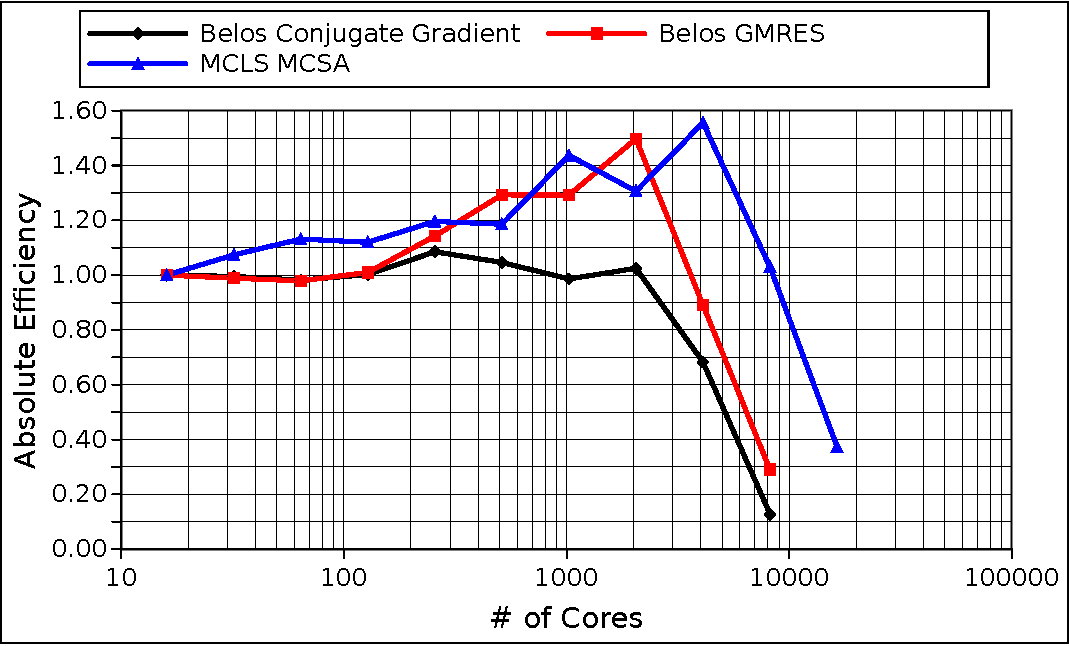
\includegraphics[width=2.4in]{titan_pure_strong.pdf}
        \end{center}
        \caption{Absolute efficiency.}
      \end{figure}

    \end{column}

  \end{columns}

  \begin{itemize}
  \item MCLS is an order of magnitude slower arithmetically.
  \item Super-linear speed-up from memory thrashing in base case.
  \item CG demonstrates poor scaling due to the cheaper iteration
    sequence
  \end{itemize}

\end{frame}

%%---------------------------------------------------------------------------%%
\begin{frame}{Weak Scaling Results}

  \begin{columns}
    \begin{column}{0.5\textwidth}

      \begin{figure}[htpb!]
        \begin{center}
          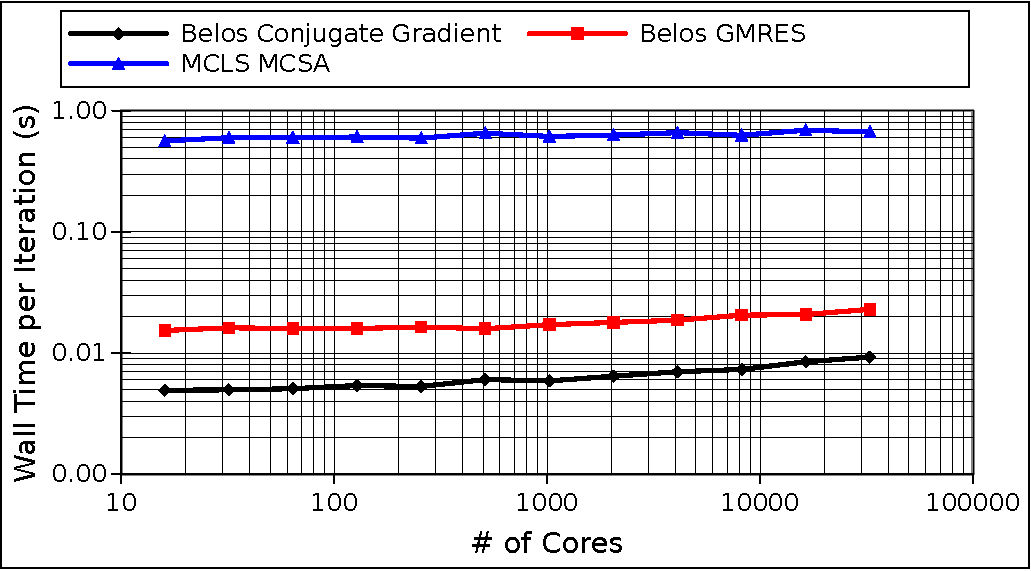
\includegraphics[width=2.3in]{titan_pure_weak_time.pdf}
        \end{center}
        \caption{Wall Time.}
      \end{figure}

      %% \begin{figure}[htpb!]
      %%   \begin{center}
      %%     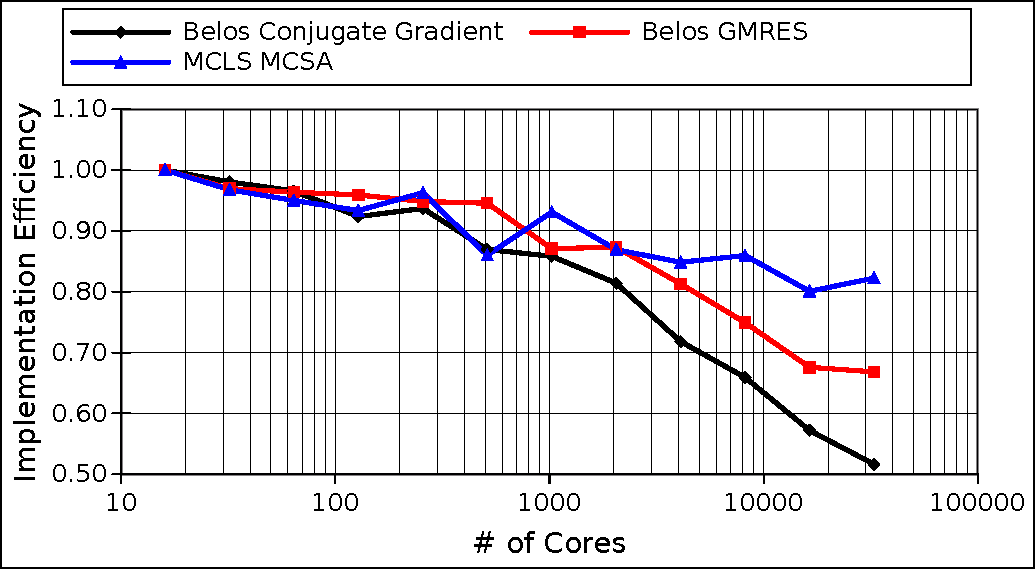
\includegraphics[width=2.3in]{titan_weak_implementation.pdf}
      %%   \end{center}
      %%   \caption{Implementation Efficiency.}
      %% \end{figure}

    \end{column}

    \begin{column}{0.5\textwidth}

      \begin{figure}[htpb!]
        \begin{center}
          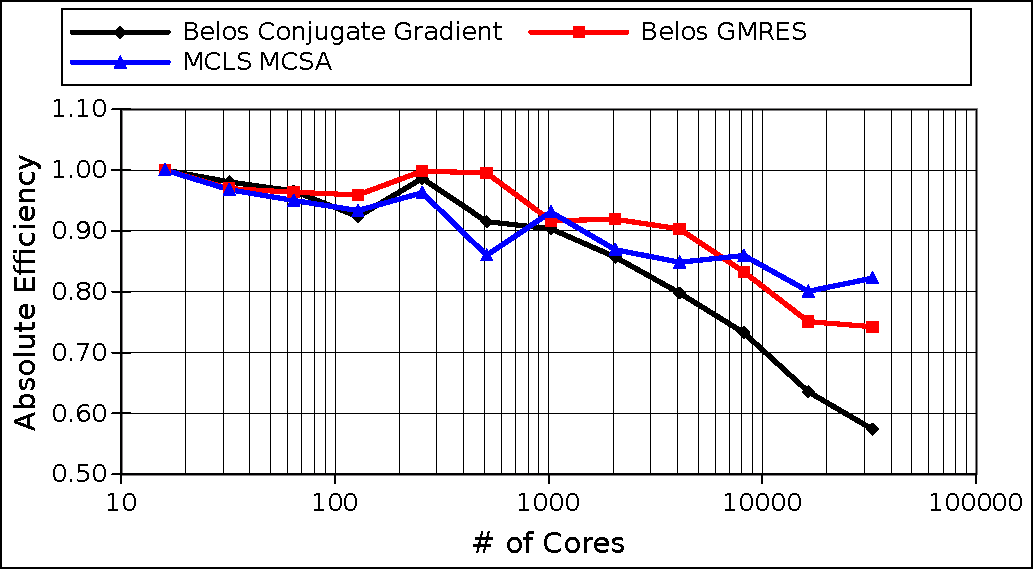
\includegraphics[width=2.3in]{titan_weak_absolute.pdf}
        \end{center}
        \caption{Absolute Efficiency.}
      \end{figure}

    \end{column}
  \end{columns}

  {\small
    \begin{itemize}
    \item Spectral radius maintained by growing the global boundary
    \item MCSA maintained constant number of iterations
    \item Krylov iteration count reduced as a function of problem size
    \end{itemize}
  }

\end{frame}

%%---------------------------------------------------------------------------%%
\begin{frame}{Strong Scaling Results with Multiple Sets}

  \textbf{Splitting:} same global number of histories as the single
  set

  \bigskip 

  \textbf{Replicating:} set-multiple of single set problem global
  histories

  \begin{columns}
    \begin{column}{0.5\textwidth}

      \begin{figure}[htpb!]
        \begin{center}
          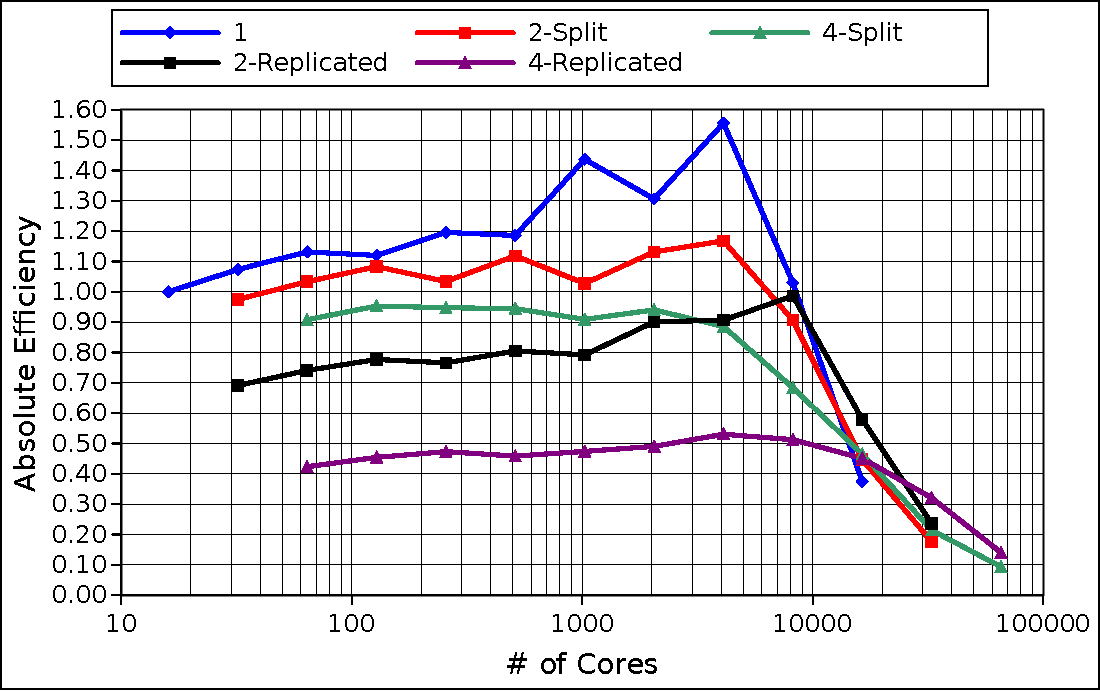
\includegraphics[width=2.35in]{titan_strong_ms_eff.pdf}
        \end{center}
        \caption{\small{Absolute efficiency relative to 16-core 1-set
            base case.}}
      \end{figure}

    \end{column}

    \begin{column}{0.5\textwidth}

      \begin{figure}[htpb!]
        \begin{center}
          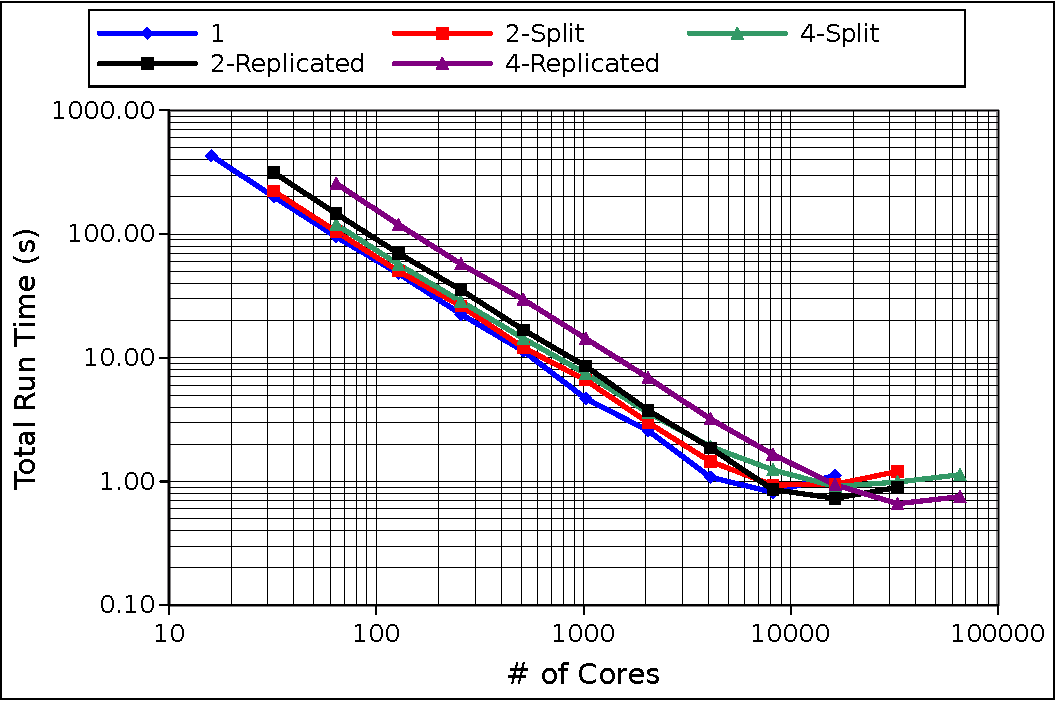
\includegraphics[width=2.35in]{titan_strong_ms_time.pdf}
        \end{center}
        \caption{\small{Wall time}}
      \end{figure}

    \end{column}
  \end{columns}

\end{frame}

%%---------------------------------------------------------------------------%%
\begin{frame}{Weak Scaling Results with Multiple Sets}

  \begin{itemize}
  \item Need to consider adding sets is a strong scaling exercise
  \item Modify the weak scaling efficiency computation to account for
    these extra resources
  \item Superposition of Monte Carlo results enhances time to solution!
  \end{itemize}

  \begin{columns}
    \begin{column}{0.5\textwidth}

      \begin{figure}[htpb!]
        \begin{center}
          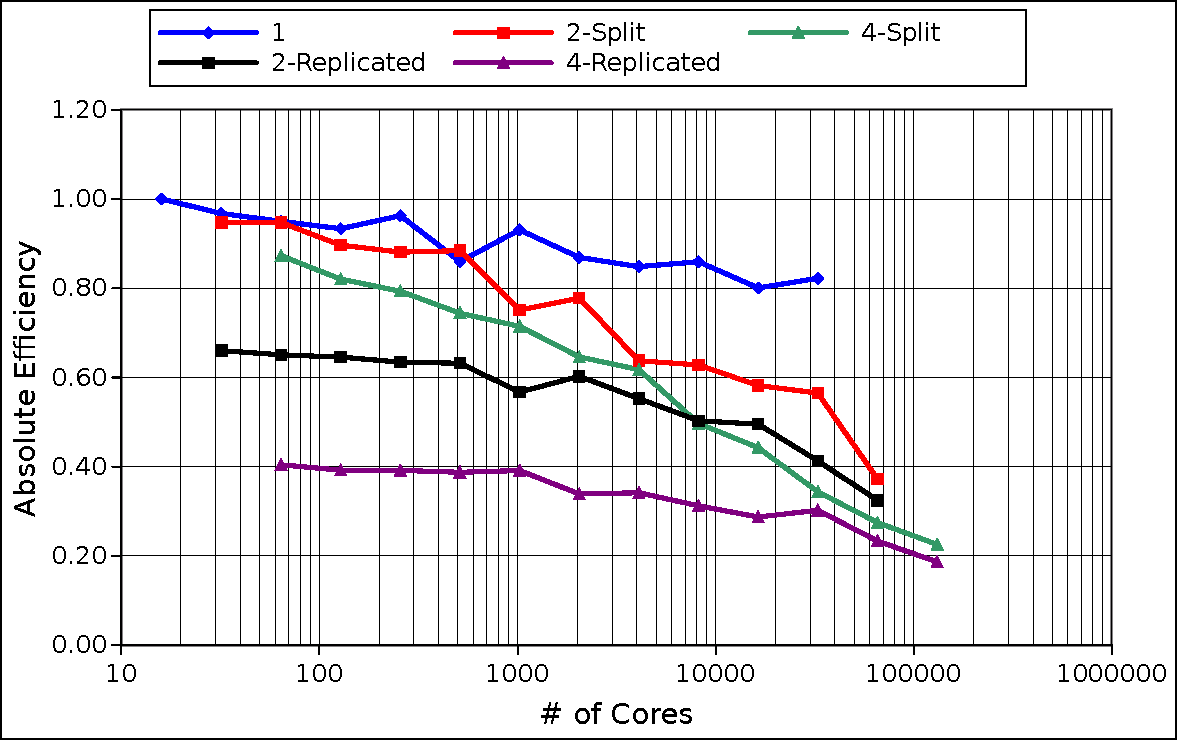
\includegraphics[width=2.4in]{titan_weak_ms_eff.pdf}
        \end{center}
        \caption{Absolute efficiency relative to 16-core 1-set base
          case.}
      \end{figure}

    \end{column}

    \begin{column}{0.5\textwidth}

      \begin{figure}[htpb!]
        \begin{center}
          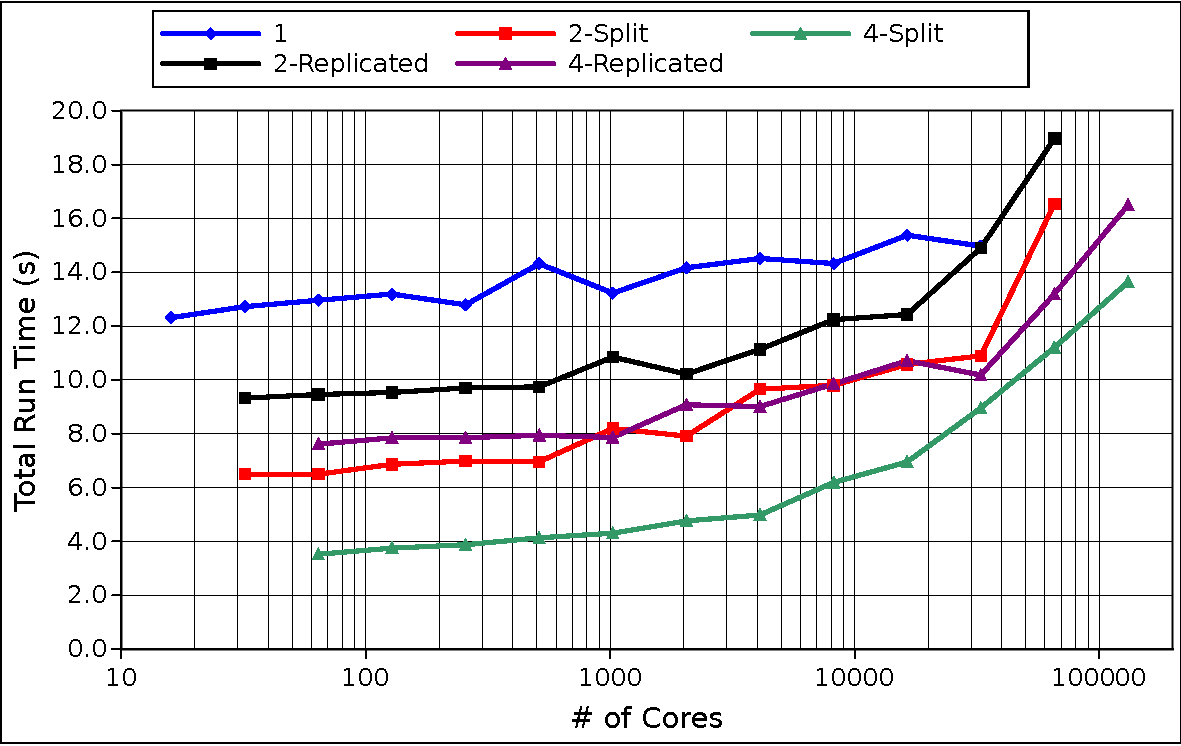
\includegraphics[width=2.4in]{titan_weak_ms_time.pdf}
        \end{center}
        \caption{Wall time.}
      \end{figure}

    \end{column}
  \end{columns}

\end{frame}

%%---------------------------------------------------------------------------%%
\begin{frame}{Scaling Results with Overlap}

  \begin{itemize}
  \item Overlap values selected based on average 'diffusion length' of
    a history in the system of 2.6 discrete states
    \bigskip
  \item Overlap eliminates communication in the Monte Carlo sequence
    but simply defers it to an overlapping tally vector reduction
  \end{itemize}

  \begin{columns}
    \begin{column}{0.5\textwidth}

      \begin{figure}[htpb!]
        \begin{center}
          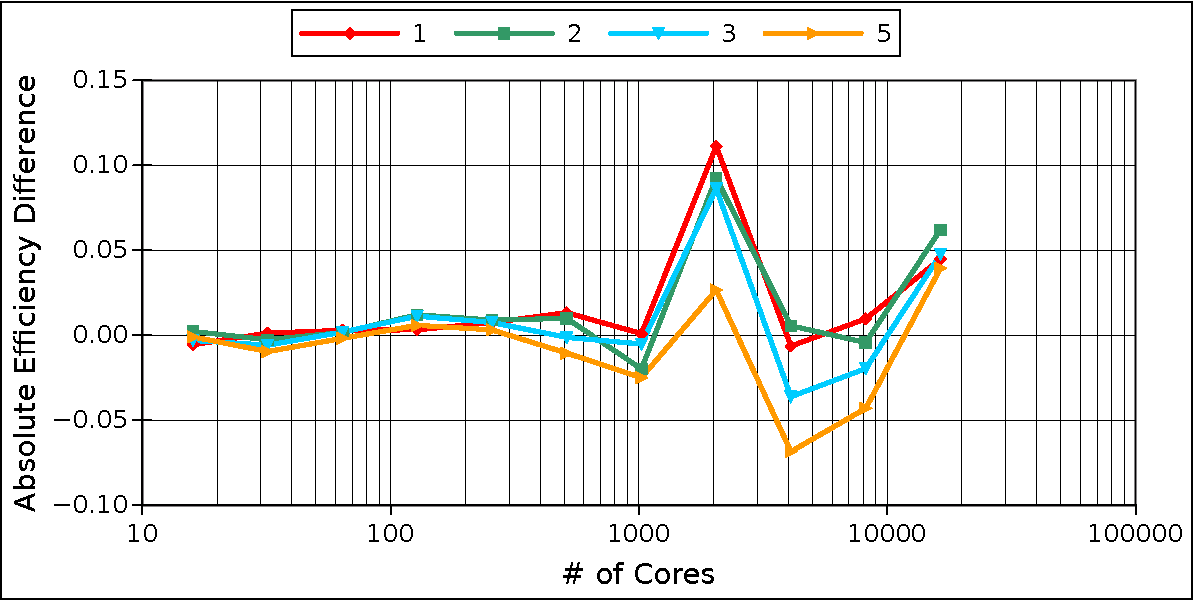
\includegraphics[width=2.4in]{titan_strong_overlap_diff.pdf}
        \end{center}
        \caption{Strong scaling efficiency difference compared to the
          0 overlap case.}
      \end{figure}

    \end{column}

    \begin{column}{0.5\textwidth}

      \begin{figure}[htpb!]
        \begin{center}
          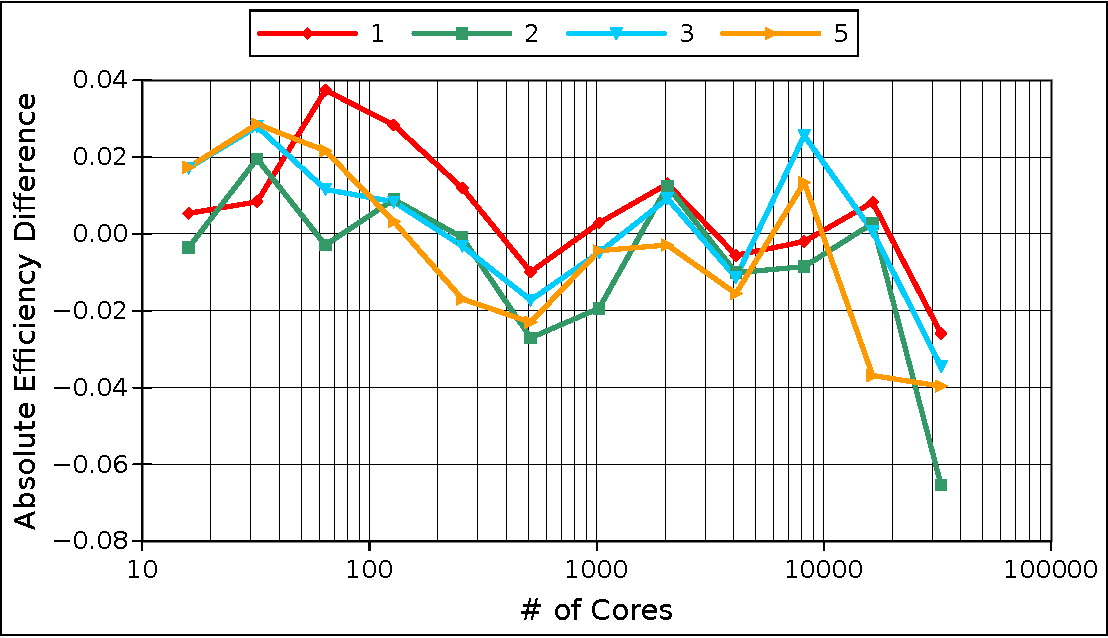
\includegraphics[width=2.4in]{titan_weak_overlap_diff.pdf}
        \end{center}
        \caption{Weak scaling efficiency difference compared to the 0
          overlap case.}
      \end{figure}

    \end{column}
  \end{columns}

\end{frame}

%%---------------------------------------------------------------------------%%
\begin{frame}{MCSA as a Stochastic Additive Schwarz Method}

  \begin{itemize}
  \item No domain-to-domain communication in Monte Carlo sequence
    \smallskip
  \item Fixed point iteration acts as a smoother
    \smallskip
  \item Observed to converge in the same number of iterations
    \smallskip
  \item Can add overlap to preserve iterative performance for more
    ill-conditioned problems
  \end{itemize}

  \begin{columns}
    \begin{column}{0.5\textwidth}

      \begin{figure}[t!]
        \begin{center}
          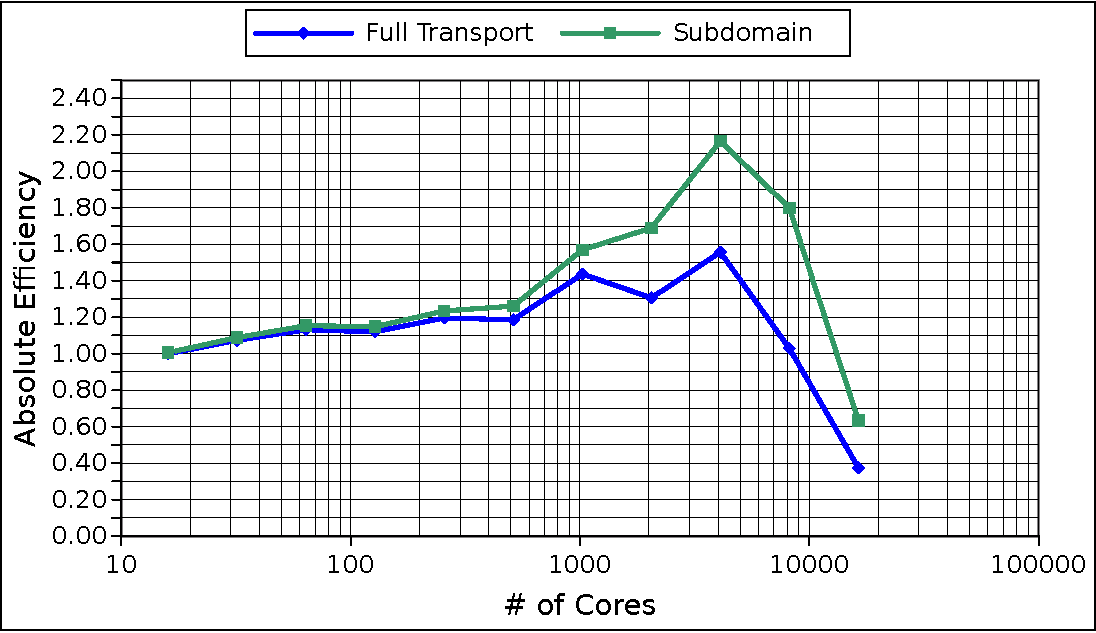
\includegraphics[width=2.35in]{titan_strong_subdomain.pdf}
        \end{center}
        \caption{Strong scaling absolute efficiency relative to full
          transport base case.}
        \label{fig:titan_strong_subdomain}
      \end{figure}

    \end{column}

    \begin{column}{0.5\textwidth}

      \begin{figure}[t!]
        \begin{center}
          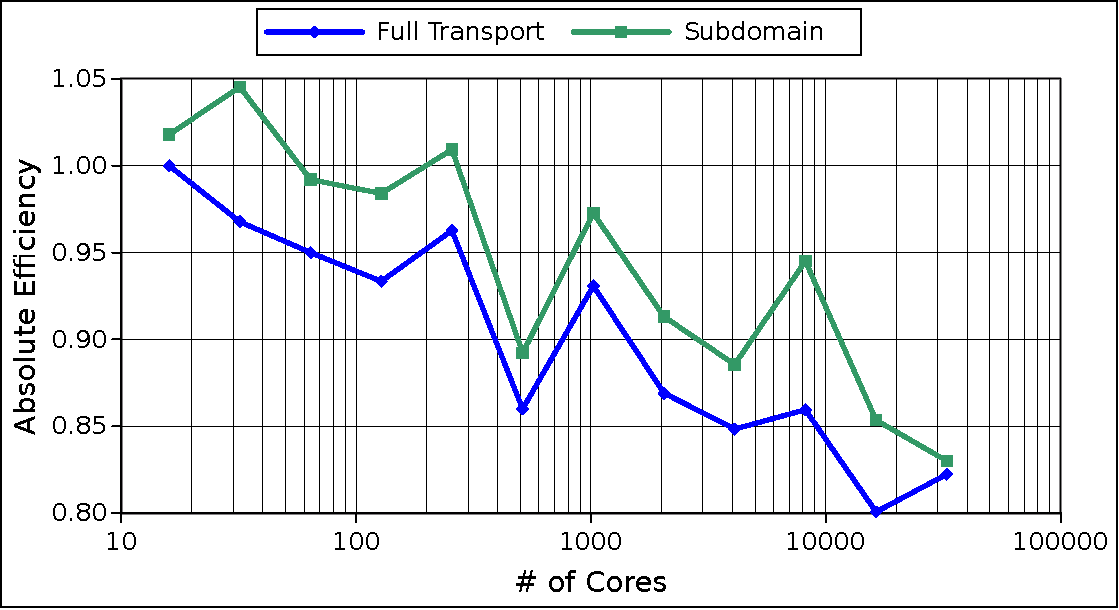
\includegraphics[width=2.35in]{titan_weak_subdomain.pdf}
        \end{center}
        \caption{Weak scaling absolute efficiency relative to full
          transport base case.}
        \label{fig:titan_weak_subdomain}
      \end{figure}

    \end{column}
  \end{columns}

\end{frame}

%%---------------------------------------------------------------------------%%
\begin{frame}{Outline}

  \begin{itemize}
  \item Introduction
    \bigskip
  \item Monte Carlo Synthetic Acceleration Methods
    \bigskip
  \item Application to Neutron Transport
    \bigskip
  \item Application to Fluid Flow
    \bigskip
  \item Parallelization of MCSA
    \bigskip
  \item \textbf{Summary}
  \end{itemize}

\end{frame}

%%---------------------------------------------------------------------------%%
\begin{frame}{MCSA Application to Neutronics Summary}

  \small{
    \begin{itemize}
    \item MCSA has been incorporated into the Exnihilo neutronics
      production code base developed at Oak Ridge National Laboratory
      \medskip
    \item MCSA can solve the asymmetric system generated by the $SP_N$
      equations
      \medskip
    \item Light water reactor problems are difficult to solve with MCSA as
      they have large spectral radii due to the neutron scattering in the
      moderator
      \medskip
    \item Advanced algebraic preconditioning strategies were applied to
      the $SP_N$ equations to obtain convergence with ILUT chosen for
      subsequent investigations
      \medskip
    \item MCSA with the reduced domain approximation was observed to
      converge in fewer iterations per eigenvalue iteration than GMRES
      for the fuel assembly criticality problem and more than
      Bi-CGStab using the same preconditioning
    \end{itemize}
  }

\end{frame}

%%---------------------------------------------------------------------------%%
\begin{frame}{MCSA Application to Fluid Flow Summary}

  \small{
    \begin{itemize}
    \item Forward-Automated Newton-MCSA (FANM) has been developed
      \medskip
    \item The FANM method has been incorporated into the Drekar
      multiphysics production code base developed at Sandia National
      Laboratories
      \medskip
    \item The FANM method has been verified to produce the same solutions
      as a production Newton-Krylov method for three difficult benchmark
      problems for the Navier-Stokes equations in different flow regimes
      and geometries
      \medskip
    \item The FANM method has better iterative performance than the
      Newton-Krylov method for convection dominated problems, converging
      in fewer linear solver iterations with the same preconditioning for
      high and low Rayleigh numbers
      \medskip
    \item The spectral radius convergence restriction on MCSA was observed
      to be a significant hindrance by preventing solutions to forced flow
      problems at high Reynolds numbers
    \end{itemize}
  }

\end{frame}

%%---------------------------------------------------------------------------%%
\begin{frame}{Parallelization of MCSA Summary}

  \small{
    \begin{itemize}
    \item The multiple-set overlapping-domain (MSOD) parallel
      algorithm for domain decomposed particle transport has been
      adapted to parallelize MCSA
      \medskip
    \item MCSA scales favorably compared to production Krylov methods for
      both strong and weak scaling cases
      \medskip
    \item Overlap in small quantities can provide parallel efficiency
      boosts of a few percent in strong scaling cases but is
      ineffective in weak scaling cases
      \medskip
    \item Multiple sets offers a means to reduce time to solution by
      solving multiple copies of the original problem and combining the
      solutions using superposition
      \medskip
    \item MCSA is most efficiently used in parallel as a stochastic
      realization of an additive Schwarz method
    \end{itemize}
  }

\end{frame}

%%---------------------------------------------------------------------------%%
\begin{frame}{Future Work}

  \begin{itemize}
  \item Shortcomings observed on real problems
    \begin{itemize}
    \item Significant optimization required to determine production
      feasibility and true scalability
    \item Explicit algebraic preconditioning methods not sufficient
    \item Spectral radius limitation is severe
    \end{itemize}
    \medskip
  \item Performance improvements
    \begin{itemize}
    \item Random walk optimizations
    \item Multiple set reduction analysis
    \item FANM forcing term and MCSA history relationships
    \end{itemize}
    \medskip
  \item Preconditioning improvements
    \begin{itemize}
    \item Variance reduction based strategy
    \item Reduced order physics/PDE models for acceleration
    \end{itemize}
    \medskip
  \item Breaking away from $\rho(\mathbf{H}) < 1$
    \begin{itemize}
    \item Monte Carlo methods of the second degree
    \end{itemize}
  \end{itemize}

\end{frame}

%%---------------------------------------------------------------------------%%
\begin{frame}{Publications}

  \small{
    \begin{enumerate}
    \item S.R. Slattery, T.M. Evans, P.P.H. Wilson, \textbf{A
      Multiple-Set Overlapping-Domain Decomposed Monte Carlo Synthetic
      Acceleration Method for Linear Systems}, \textit{Joint
      International Conference on Supercomputing in Nuclear
      Applications and Monte Carlo 2013 (SNA+MC 2013), Paris, France,
      October 27-31, 2013. Accepted for oral presentation.}
      \medskip
    \item S.R. Slattery, T.M. Evans, P.P.H. Wilson, \textbf{A Spectral
      Analysis of the Domain Decomposed Monte Carlo Method for Linear
      Systems}, \textit{International Conference on Mathematics and
      Computational Methods Applied to Nuclear Science \& Engineering
      (M\&C 2013), American Nuclear Society, Sun Valley, ID, May 5-9,
      2013.}
      \medskip
    \item T.M. Evans, S.W. Mosher, S.R. Slattery, S.P. Hamilton,
      \textbf{A Monte Carlo Synthetic-Acceleration Method for Solving
        the Thermal Radiation Diffusion Equation}, \textit{Journal of
        Computational Physics, Submitted.}
    \end{enumerate}
  }
\end{frame}

%%---------------------------------------------------------------------------%%
\begin{frame}{Thank You}

  \begin{itemize}
  \item Paul Wilson
  \item Tom Evans
  \item Roger Pawlowski
  \item CASL, ORNL, Sandia, OLCF
  \end{itemize}

\end{frame}

%%---------------------------------------------------------------------------%%

\end{document}
